 \documentclass[12pt,a4paper]{report}
\usepackage[a4paper,vmargin={1in,1in},hmargin={1.25in,1in}]{geometry}	% Setup of page size,margins
\usepackage{graphics}
\usepackage[font=small,labelfont=bf]{caption}
\usepackage{epsfig}
\usepackage{tabularx}
%\usepackage{algpseudocode}
%\usepackage{algorithm}
\usepackage{subfigure}  
\usepackage[titletoc]{appendix}
\renewcommand{\appendixname}{Annexure}
\usepackage{multirow}
\usepackage{fancyhdr}		% For special customization of headers and footers
\usepackage{fancybox}		% For formatting of cover page5
\usepackage{amsmath}    	% For  mathematical formulae
\usepackage{amsfonts}
\usepackage{amssymb}
\usepackage{textcomp}
\usepackage{setspace}		% For adjusting line spacing 
\usepackage{pdfpages}
\usepackage[square, comma, sort&compress,numbers]{natbib} % For customizing citations
%\usepackage[pdftex]{hyperref}	% For having working URLs for references 
\usepackage[colorlinks=true,linkcolor=blue,urlcolor=blue]{hyperref}
\usepackage[UKenglish]{isodate}
\usepackage[intoc]{nomencl}
\usepackage{multirow} 		  	% for row spannig in table environment
\usepackage{xcolor}
\definecolor{light-gray}{gray}{0.95}
\usepackage{footnote} 			% this package conflicts with xcolor.  So keep its order as is
\makenomenclature
\onehalfspacing
\author{}
 \title{ALERTO}
\begin{document}
\pagenumbering{roman}
\pagestyle{empty}
%------------------------------------------------------------------------------
%   Cover Page starts here
%------------------------------------------------------------------------------
\newpage
\pagestyle{empty}
\pagenumbering{gobble}
%\thisfancypage{cmds1}{cmds2}
\thisfancyput(-0.0 in, -10.0 in) {\setlength{\unitlength}{1 in}\framebox(6.7,10.2)}

\begin{center}
	\vspace*{0.2 in}
	\textbf{\large{SAVITRIBAI PHULE PUNE UNIVESITY}}\\
  \vspace*{0.25 in}
\textbf{A PROJECT REPORT ON}
\vspace{0.05 in}
  \end{center}
\vspace{0.05 in}
	\begin{center}
		\textbf{\large{ALERTO}} \\
	\end{center}
	
	\vspace{0.1 in}
	\begin{center}
	SUBMITTED TOWARDS THE PARTIAL FULFILLMENT OF THE REQUIREMENTS OF
\end{center}
	\vspace{0.1 in}
	\begin{center}
			\textbf{BACHELOR OF ENGINEERING(Computer Engineering)}
     	\end{center}
     \vspace{0.3 in}
		\begin{center}
	    BY
	\end{center}
	
	
	\begin{flushleft}
		\begin{flushleft}
\hspace{1.7in}\textbf{Mihika Deshpande     403005}\\
\hspace{1.7in}\textbf{Tarini Parihar}    
 \hspace{0.3in}\textbf{  403010}\\
\hspace{1.7in}\textbf{Ruchi Jain}\hspace{0.65in}\textbf{           403014}\\
\hspace{1.7in}\textbf{Zindagi}\hspace{0.94in}\textbf{              403029}\\
\end{flushleft}
	\end{flushleft}
	\vspace{0.2 in}
	
		\begin{center}
			\textbf{SPONSORED BY}\\
			\vspace{0.05 in}
			\textbf{ RAJA SOFTWARE LABS PVT.LTD.}
		\end{center}
		\vspace{0.05 in}
		
	\begin{center}
	  \textbf{UNDER THE GUIDANCE OF}\\
	  \vspace{0.075 in}
	 \textbf{ Prof. S. R. VIJ}(Internal Guide)\\
	  \textbf{Mr. PRAKHAR AJABE }(External Guide)
	\end{center}
		%\vspace{0.2 in}
		
		\vspace{0.3 in}
\begin{center}

\includegraphics[width=3cm]{mitlogo}
\end{center}

		\begin{center}
	  \textbf{Department Of Computer Engineering}\\
\bf{MAEER’s MAHARASHTRA INSTITUTE OF TECHNOLOGY} \\
\textbf{Kothrud, Pune 411 038}\\
\textbf{2015-2016}
	\end{center}
%------------------------------------------------------------------------------
%  Cover ends here
%------------------------------------------------------------------------------

%------------------------------------------------------------------------------
%  Certificate starts here
%------------------------------------------------------------------------------
\newpage
\pagestyle{empty}
 %\thispagestyle{empty}
	\pagenumbering{gobble}
	\thisfancyput(-0.0 in, -10.0 in) {\setlength{\unitlength}{1 in}\framebox(6.7,10.2)}
\begin{center}
\begin{figure}[h]
\centering
\includegraphics[width=1.5 cm]{MITLogo}
\end{figure}
 MAHARASHTRA ACADEMY OF ENGINEERING AND EDUCATIONAL RESEARCH\textquoteright S\\ \bf \vspace {0.001 in}MAHARASHTRA INSTITUTE OF TECHNOLOGY\\ PUNE\\\vspace {0.001 in} DEPARTMENT OF COMPUTER ENGINEERING\\
\vspace {0.0001 in}
\end{center}
\vspace{0.0005 in}
\begin{center}
\textbf{\underline{C E R T I F I C A T E}}\\
\vspace{0.0005 in}
\end{center}
		\noindent
  				\setlength{\baselineskip}{1.45\baselineskip}
	\begin{center}
This is to certify that \\
\textbf{\large ALERTO}\\
Submitted by\\
	\begin{flushleft}
		\begin{flushleft}
			\hspace{1.7in}\textbf{Mihika Deshpande     403005}\\
			\hspace{1.7in}\textbf{Tarini Parihar}    
			\hspace{0.3in}\textbf{  403010}\\
			\hspace{1.7in}\textbf{Ruchi Jain}\hspace{0.65in}\textbf{           403014}\\
			\hspace{1.7in}\textbf{Zindagi}\hspace{0.94in}\textbf{              403029}\\
		\end{flushleft}
	\end{flushleft}
	
	is a bonafide work carried out by Students under the supervision of Prof. S. R. Vij and it is submitted towards the partial fulfillment of the requirement of Bachelor of Engineering (Computer Engineering).
		\begin{center}
	Prof. S. R. Vij \hspace{0.95 in} \hspace{0.95 in} \hspace{0.95 in}Dr. V. Y. Kulkarni\\
	Internal Guide \hspace{0.9 in} \hspace{0.9 in} \hspace{0.9 in} \hspace{0.9 in} H.O.D.\\
	Dept. of Computer Engg. \hspace{0.7 in} \hspace{0.7 in} \hspace{0.7 in} Dept. of Computer Engg.\\

		Dr. L. K. Kshirsagar\\
		Principal\\
		Maharashtra Institute of Technology
	
	\vspace{0.5 in}
	
	Signature of Internal Examiner \hspace{0.7 in} \hspace{0.7 in} Signature of External Examiner
\end{center}

\pagenumbering{roman}
\begin{center}
	\textbf{PROJECT APPROVAL SHEET}\\
	\vspace{0.2 in}
	A Project title\\
	\vspace{0.1 in}
	\textbf{ALERTO}\\
	\vspace{0.15 in}
	Is successfully completed by\\
	\begin{flushleft}
		\begin{flushleft}
			\hspace{1.7in}\textbf{Mihika Deshpande     403005}\\
			\hspace{1.7in}\textbf{Tarini Parihar}    
			\hspace{0.3in}\textbf{  403010}\\
			\hspace{1.7in}\textbf{Ruchi Jain}\hspace{0.65in}\textbf{           403014}\\
			\hspace{1.7in}\textbf{Zindagi}\hspace{0.94in}\textbf{              403029}\\
		\end{flushleft}
	\end{flushleft}
	at\\
	\vspace{0.1 in}
\textbf{DEPARTMENT OF COMPUTER ENGINEERING}\\
	\vspace{0.1 in}
	\textbf{MAHARASHTRA INSTITUTE OF TECHNOLOGY}\\
	\vspace{0.1 in}
	\textbf{SAVITRIBAI PHULE PUNE UNIVERSITY,PUNE}\\
	\vspace*{0.1 in}
	\textbf{ACADEMIC YEAR 2015-2016}\\
	\vspace{0.9 in}
	Prof. S. R. Vij \hspace{0.9 in}\hspace{0.9 in} \hspace{0.9 in}Dr. V. Y. Kulkarni\\
	Internal Guide \hspace{0.6 in}\hspace{0.6 in}\hspace{0.6 in} \hspace{0.6 in} \hspace{0.6 in}\hspace{0.6 in} H.O.D.\\
	Dept. of Computer Engg. \hspace{0.7 in} \hspace{0.7 in} \hspace{0.6 in} Dept. of Computer Engg.\\
\end{center}
\singlespace

	\end{center}

%------------------------------------------------------------------------------
%  Certificate ends here
%------------------------------------------------------------------------------
%------------------------------------------------------------------------------
%  Abstract starts here
%------------------------------------------------------------------------------
%\newpage
%\addcontentsline{toc}{section}{ABSTRACT}

\begin{abstract}
	
	\begin{normalsize}
		
		\hspace{6mm} The proposed application targets at implementing a system which will enable the end-users to make their life easy. We are using technologies like wearable device, Bluetooth LE and Android SDK.The system will help the users to get rid of the constant urge to check their phone instead it will notify them whenever an important call or message is coming on their phone\\
		
		We are using Bluetooth low energy instead of bluetooth to save the battery which is an important issue in Android phones.We have a device called "ALERTO" which needs to be synced to our application so that it can alert the user.\\
		
		\textbf{Keywords:}\\ 
		Bluetooth LE, Wearable Device,Alerto.
		
	\end{normalsize}
\end{abstract}
%------------------------------------------------------------------------------
%  Abstract ends here
%------------------------------------------------------------------------------
\newpage
%\addcontentsline{toc}{section}{ACKNOWLEDGMENT}
\pagestyle{plain}           %For displaying roman page nos
\begin{center}
\bf ACKNOWLEDGEMENT
\end{center}
\hspace*{0.6cm}It gives us great pleasure in presenting the preliminary project report on `ALERTO'.\\

We would like to take this opportunity to thank our internal guide Prof. S. R. Vij
for giving us all the help and guidance we needed. We are really grateful for
her kind support. Her valuable suggestions were very helpful.\\

We are also grateful to Dr. V. Y. Kulkarni, Head of Computer Engineering Department, Maharashtra Institute of Technology, Pune for her indispensable support, suggestions.\\

In the end our special thanks to Mr. Prakhar Ajabe, our external guide for providing constant support and guidance  for our Project. We are grateful to him for giving his valuable time and knowledge.


\begin{flushleft}
\hspace{3.7in}Mihika Deshpande\\
\hspace{3.7in}Tarini Parihar\\
\hspace{3.7in}Ruchi Jain\\
\hspace{3.7in}Zindagi\\
\hspace{3.7in}(B.E. Computer Engineering)\\
\end{flushleft}

%------------------------------------------------------------------------------
%  Acknowledgement ends here


%------------------------------------------------------------------------------
%  TOC starts here
%------------------------------------------------------------------------------
\newpage

\tableofcontents
%------------------------------------------------------------------------------
%  List of Figures,tables starts here
%------------------------------------------------------------------------------

\newpage
{\setlength{\baselineskip}{1.5\baselineskip}
\listoffigures
%\addcontentsline{toc}{section}{List of Figures}
}
\newpage
{\setlength{\baselineskip}{1.5\baselineskip}
\listoftables
%\addcontentsline{toc}{section}{List of Tables}
}


%------------------------------------------------------------------------------


%\begin{center}
\chapter{\bf{SYNOPSIS}}
%\end{center}
\pagenumbering{arabic}     %For displaying arabic(1,2,3 ..) page nos
\pagestyle{fancy}
\fancyhead[RO]{\textit{\begin{small}ALERTO\end{small}}}
\fancyhead[LO]{\textit{\begin{small}PROJECT\end{small}}}
\renewcommand{\footrulewidth}{0.3pt}
\fancyfoot[RO]{\textit{\begin{small}Dept. of Computer Engg.\end{small}}}
\fancyfoot[LO]{\textit{\begin{small}MIT, Pune .\end{small}}}

\newpage
\section{PROJECT TITLE}
The title of our project is `ALERTO'

\section{PROJECT OPTION}
The option of our project is Industry sponsored

\section{INTERNAL GUIDE}
The internal guide of our project is  Prof. S. R. Vij

\section{SPONSORSHIP AND EXTERNAL GUIDE}
Our project is sponsored by Raja Software Pvt. Ltd. under the guidance of Mr. Prakhar Ajabe.

\section{TECHNICAL KEYWORDS}
\textbf{A.Hardware}
\begin{itemize}
	\item Alerto(The wearable device)
	\item Android phone
\end{itemize}
\textbf{B.Architecture}
\begin{itemize}
	\item Client Server Architecture
	\item Database Connectivity
\end{itemize}
\textbf{C.Networking}
\begin{itemize}
	\item Bluetooth LE
\end{itemize}
\textbf{D.Network Protocols}
\begin{itemize}
	\item Broadcast 
	\item Send and Receive
\end{itemize}

\section{PROBLEM STATEMENT} 
 Development of an android application for a wearable device called `Alerto', that detects notifications for calls, messages and conversations of any android devices  using Bluetooth Low Energy technology and alert users using the device.
 
\section{ABSTRACT}
The proposed application targets at implementing a system which will enable the end-users to make their life easy. We are using technologies like wearable device, Bluetooth LE and Android SDK.The system will help the users to get rid of the constant urge to check their phone instead it will notify them whenever an important call or message is coming on their phone.

We are using Bluetooth low energy instead of bluetooth to save the battery which is an important issue in Android phones.We have a device called "ALERTO" which needs to be synced to our application so that it can alert the user.

\section{GOALS AND OBJECTIVES}
\begin{enumerate}
	\item To free the user from the constant urge to check the phone.
	\item To provide the user with a user-friendly environment so that user becomes technologically accustomed.
	\item To inform the user when the phone is out of reach.
	\item To let the user know  when a notification from an important contact has arrived.
\end{enumerate}

\section{RELEVANT MATHEMATICS ASSOCIATED WITH THE PROJECT}
\subsection{MATHEMATICAL MODEL}
	A mathematical model is a description of system using mathematical concepts and language.  A model may help to explain a system and to study the effects of different components, and to make predictions about behaviour.
	
	Mathematical models can take many forms, including but not limited to dynamical systems, statistical models, differential equations, or game theoretic models. These and other types of models can overlap, with a given model involving a variety of abstract structures. In general, mathematical models may include logical models.
	
	In many cases, the quality of a scientific field depends on how well the mathematical models developed on the theoretical side agree with results of repeatable experiments. Lack of agreement between theoretical mathematical models and experimental measurements often leads to important advances as better theories are developed.
	
	Mathematical Model for Android Application `Alerto':
	\begin{itemize}
		\item I: Set of Inputs
        \item O: Set of outputs
		\item F: Functions
		\item Sc: Success cases
		\item Fc: Failure cases\\
	\end{itemize}
	
\begin{itemize}
\item I= \{I1, I2\}
where,
\begin{itemize}
\item I1: Installation of the Android application ‘Alerto’
\item I2: Execution of the application
\end{itemize}
\item O: \{O1, O2\}
where,
\begin{itemize}
\item O1: List of available Alertos
\item O2: Connection established with a particular Alerto.
\end{itemize}
\item F: \{F1, F2, F3, F4, F5\}
where,
\begin{itemize}
\item F1: Get started with the application.
\item F2: Turn on Bluetooth.
\item F3: Scan for available Alerto devices in range.
\item F4: Connect with specific Alerto.
\item F5: Once desired notification arrives on smart phone, the particular Alerto vibrates.
\end{itemize}
\item Sc: \{Sc1, Sc2\}
where,
\begin{itemize}
\item Sc1: Connection established.
\item Sc2: Alerto vibrates.
\end{itemize}
\item Fc: \{Fc1, Fc2, Fc3, Fc4, Fc5\}
where,
\begin{itemize}
\item Fc1: Application not working.
\item Fc2: Installation error.
\item Fc3: Alerto devices invisible.
\item Fc4: Connection establishment error.
\item Fc5: Vibration doesn’t occur
\end{itemize}
\end{itemize}
\begin{figure}[!h]
	\begin{center}
			\scalebox{0.7}{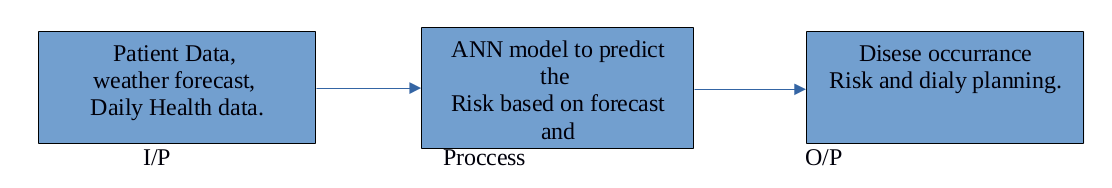
\includegraphics{math.png}}
			\caption{Mathematical model}
	\end{center}
\end{figure}
\section{NAMES OF CONFERENCES / JOURNALS WHERE PAPERS CAN BE PUBLISHED}
\begin{itemize}
\item IEEE/ACM Conference/Journal 1
\item Conferences/workshops in IITs
\item Central Universities or SPPU Conferences
\item IEEE/ACM Conference/Journal 2
\end{itemize}

\section{PLAN OF PROJECT EXECUTION}

\begin{table}[h]
	
	\caption {Plan of Project Execution}
	\center
	\begin{tabular}{ |p{3cm}|p{3cm}|p{3cm}|p{3cm}|  }
		
		\hline
		From & To & Task & Status\\
		\hline
		27\textendash06\textendash2015 & 30\textendash06\textendash2015 & Group Formation and finalization &  Done\\
		\hline
		
		01\textendash07\textendash2015 & 15\textendash07\textendash2015 & Topic Search & Done\\
		\hline
		
		16\textendash07\textendash2015 & 20\textendash07\textendash2015 & Preliminary Information Gathering &  Done\\
		\hline
		
		21\textendash07\textendash2015 & 28\textendash07\textendash2015 & Project Dicsussion with Project Coordinator and topic finalization &  Done\\
		\hline
		
		01\textendash08\textendash2015 & 04\textendash08\textendash2015 & Synopsis  preparation and submission &  Done\\
		\hline
		
		25\textendash08\textendash2015  & 30\textendash08\textendash2015    & Detailed Literature Survey &  Done\\
		
		
		19\textendash09\textendash2015	&	24\textendash09\textendash2015 & . & .\\
		\hline
		
		25\textendash09\textendash2015 & 06\textendash10\textendash2015 & Preparing Interim report &  Done\\
		\hline
		
		20\textendash12\textendash2015 & 02\textendash01\textendash2016 & Language Study &  Done\\
		\hline
		
		03\textendash01\textendash2016 & 20\textendash01\textendash2016 & Android and Bluetooth LE Study &  Done\\
		\hline
		
		21\textendash01\textendash2016 & 04\textendash03\textendash2016 & Coding and Implementation &  Done\\
		\hline
		
		05\textendash03\textendash2016 & 21\textendash04\textendash2016 & Testing &  Done\\
		\hline
		
		13\textendash04\textendash2016 & 21\textendash04\textendash2016 & Final Documentation &  Done\\
		\hline
		
		25\textendash04\textendash2016 & 20\textendash05\textendash2016 & Final Project Report &  Done\\
		\hline		
	\end{tabular}
	
\end{table}



\chapter{\bf{TECHNICAL KEYWORDS}}
\newpage

\section{AREA OF PROJECT}
The area of our project is Mobile Application.
\section{TECHNICAL KEYWORDS}
\textbf{A.Hardware}
\begin{itemize}
	\item Alerto(The wearable device)
	\item Android phone
\end{itemize}
\textbf{B.Architecture}
\begin{itemize}
	\item Client Server Architecture
	\item Database Connectivity
\end{itemize}
\textbf{C.Networking}
\begin{itemize}
	\item Bluetooth LE
\end{itemize}
\textbf{D.Network Protocols}
\begin{itemize}
	\item Broadcast 
	\item Send and Receive
\end{itemize}

\chapter{INTRODUCTION}
\newpage

\section{PROJECT IDEA}
The proposed application targets at implementing a system which will enable the end-users to make their life easy. We are using technologies like wearable device, Bluetooth LE and Android SDK.The system will help the users to get rid of the constant urge to check their phone instead it will notify them whenever an important call or message is coming on their phone.

\section{MOTIVATION OF THE PROJECT}
Many times a situation has occured where a call or message was missed while doing some important work and we were unable to check it at that time. Hence we decided to create an application which will help us to avoid this inconvenience. 

\section{LITERATURE SURVEY}
\textbf{1.Modeling Neighbor Discovery in Bluetooth Low Energy Networks\\ Jia Liu, Member, IEEE, Canfeng Chen, Member, IEEE, and Yan Ma, Member, IEEE COMMUNICATIONS LETTERS, VOL. 16, NO. 9, SEPTEMBER 2012}

An analytical model is proposed for 3-channel-based neighbor discovery in Bluetooth Low Energy(BLE) networks. The model can be used to determine some important
performance metrics, such as average latency or average energy consumption during the course of discovering neighbors. Since intermittent connections are frequently encountered in practical scenarios of BLE, the modeling results can provide a
beneficial guidance to customize advertising or scanning behavior towards user desired performance.

\textbf{2.Energy Analysis of Device Discovery for Bluetooth Low Energy\\
    Jia Liu, Member, IEEE, Canfeng Chen, Member, IEEE, and Yan Ma, Member, IEEE
	}
	
	Bluetooth Low Energy (BLE) is drawing more and 	more attention due to its recent appearance in consumer 	electronic products. As a low-power wireless solution, BLE 	provides attractive energy performance that makes it 	particularly suitable for portable, battery-driven electronic devices. Although there are some prior arts focusing on BLE energy performance, it still lacks a thorough study on the important aspect of device discovery. Such energy cost,
	introduced by intermittent scanning or connection setup, could seriously affect the battery endurance ability of the devices. In this paper, quantitative analysis on the neighbor discovery energy for BLE is persented. The modeling results that built upon measurement of CC2541 Mini-Development Kit have been
	validated quite accurate via extensive experiments. In addition, several interesting conclusions are found while investigating the achieved energy model, which may provide precious guidelines to the design of energy-efficient applications for BLE.

\textbf{3.Advertising semantically described physical items with Bluetooth Low Energy beacons	2nd Mediterranean Conference on Embedded Computing ,,/" MECD - 2013}

Enabling smart applications to access information about the physical world in a machine interpretable format is a high priority in the Internet of Things (loT) related research. In this paper, we present a novel approach for advertising
information related to physical objects in the user vicinity. There are three distinctive features in the approach. First, ubiquitous codes (ucodes) are used for providing globally unique identifiers for the physical objects. Second, using Bluetooth Low Energy beacons for broadcasting the identifiers of the physical objects. 

Third, the information related to the physical object is represented with semantic technologies.
\newpage
\textbf{4.Wapplet: A Media Access Framework for	Wearable Applications\\
	Takeshi Iwamoto1, Nobuhiko Nishio1, and Hideyuki Tokuda1,2\\
	1. Graduate School of Media and Governance, Keio University, Japan
	{iwaiwa, vino, hxt}@ht.sfc.keio.ac.jp\\
	2.Faculty of Environmental Information, Keio University, Japan}

This paper presents a new framework for constructing applications for wearable computers. We do not consider wearable computing merely as a single self-confined system. Rather, wearable computing can be treated as a cooperative application with information surrounding a person and various devices attached to him/her. We have developed a framework of such wearable computing called “Wapplet.” Wapplet provides
adaptation to the availability of devices as well as a systematic scheme of constructing applications for wearable computing. In this paper, we describe the design and implementation of Wapplet, and show its prototype system.

\textbf{5.Wearable Electronics Sensors: Current Status and Future Opportunities
	Anindya Nag and Subhas Chandra Mukhopadhyay Massey University, Palmerston North, New Zealand}

The technological advancement in the past three decades has impacted our lives and wellbeing significantly. Different aspects of monitoring our physiological parameters are considered. Wearable sensors are one of its most important areas that have an ongoing trend and have a huge tendency to rise in the future. The wearable sensors are the externally used devices attached to any individual to measure physiological parameters of interest. The range of wearable sensors varies from minuscule to large scaled devices physically fitted to the user operating on wired or wireless terms. Many common diseases affecting large number of people notably gait abnormalities, Parkinson’s disease are analysed by the wearable sensors. The use of wearable sensors has got a better prospect with improved technical qualities and a better understanding of the currently used research methodologies. This chapter deals with the overview of the current and past means of wearable sensors with its associated protocols used for communication. It concludes with the ways the currently dealt wearable sensors can be improved in future.


\chapter{PROBLEM DEFINITION AND SCOPE}
\newpage
\section{PROBLEM STATEMENT}
Development  of  an  android  application  for  a  wearable device  called  ‘Alerto’,  that  detects  notifications  for  calls,  messages  and conversations  of  your  android  devices  using  Bluetooth  Low Energy technology and alert users using the device.

\subsection{Goals and Objectives}
\begin{enumerate}
	\item To free the user from the constant urge to check the phone.
	\item To provide the user with a user-friendly environment so that user becomes technologically accustomed.
	\item To inform the user when the phone is out of reach.
	\item To let the user know  when a notification from an important contact has arrived.
\end{enumerate}

\subsection{Statement of Scope}
We describe what features are in the scope of the software and what are not in scope of the software to be developed.
\begin{enumerate}
	\item	Notifications for Incoming Calls \\
	The user will feel it vibrate when someone they have chosen as important is trying to reach them.
	\item	Notifications for Incoming Texts \\
	 The user will feel it vibrate when someone they have chosen as important is trying to text them.
	\item	Notifications for When The User Leave Their Phone Behind \\
	Alerto has a built-in wireless tether. When the user is about to leave their phone behind, Alerto will vibrate to warn them.
	\item	No Cables, No Buttons, No Recharging \\
	Since Alerto never needs charging, just leave it with other things. Alerto will remind the user when it needs a new battery.
\end{enumerate}

\section{MAJOR CONSTRAINTS}
\begin{enumerate}
	\item	The android version used in the app should be higher than Jelly\_bean\_MR2(4.3+)
	\item	The distance between the Alerto device and Smartphone should be within Bluetooth LE range.
	\item	App requires access to contact details, Bluetooth information, Device ID and call information
\end{enumerate}


\section{METHODOLOGIES OF PROBLEM SOLVING AND EFFICIENCY ISSUES}
A problem can be solved by many different solutions. The methodologies of problem solving considers the performance parameters for each approach. Thus considering the efficiency issues.
\begin{enumerate}
	\item Our project is based on Android operating system  but it can be implemented on other operating systems as well. However we have selected Android because it is much more popular in comparison to other OS which increases the usability of our application.
	\item Bluetooth Low energy uses less amount of battery power as compared to classic Bluetooth devices. Hence using this technology helps to reduce power consumption and increase  battery life. Thus we have used this technology for our application
\end{enumerate}

\section{OUTCOME}
We have implemented an application in Android with a wearable device which alerts the users about incoming notifications.

\section{HARDWARE RESOURCES REQUIRED}
\begin{enumerate}
	\item	400MB Hard disk+1GB for Android SDK, emmulator system images and caches
	\item	Alerto device(Wearable)
	\item	2GB RAM minimum,4GB RAM recommended
	\item	Intel Processor with support for Intel VT-x, Intel EM64T(Intel 64)
	\item	Computer  with windows Vista/7/8.
	
\end{enumerate}

\section{SOFTWARE RESOURCES REQUIRED}

\begin{itemize}
	\item Platform: Android SDK
\item  Operating System: Android
\item  Programming Language: Java, XML.
\end{itemize}

\chapter{PROJECT PLAN}
\newpage
\section{PROJECT ESTIMATES}
In "The Waterfall" approach, the whole process of software development is divided into separate phases. In Waterfall model, typically, the outcome of one phase acts as the input for the next phase sequentially.

\begin{figure}[!h]
	\begin{center}
		\scalebox{0.7}{\includegraphics{sdlc_waterfall_model.jpg}}
		\caption{Waterfall model}
	\end{center}
\end{figure}

The sequential phases in Waterfall model are: 
\begin{itemize}
\item \textbf{Requirement Gathering and analysis:}

 All possible requirements of the system to be developed are captured in this phase and documented in a requirement specification document.
\begin{itemize}
\item \textbf{Hardware Requirements:}
\begin{itemize}
\item 400MB Hard disk+1GB for Android SDK, emmulator system images and caches
\item Alerto device(Wearable)
2GB RAM minimum,4GB RAM recommended
\item Intel Processor with support for Intel VT-x, Intel EM64T(Intel 64)
\item Computer  with windows Vista/7/8.
\end{itemize}
\item \textbf{Software Requirements:}
\begin{itemize}
\item Platform: Android SDK
\item Operating System: Android
\item Programming Language: Java, XML.
\end{itemize}
\end{itemize}
\item \textbf{System Design:} The requirement specifications from first phase are studied in this phase and system design is prepared. System Design helps in specifying hardware and system requirements and also helps in defining overall system architecture.
\begin{itemize}
\item The App will be developed using Android SDK
\item The app is created using Android/Java
\end{itemize}
\item \textbf{Implementation:} With inputs from system design, the system is first developed in small programs called units, which are integrated in the next phase. Each unit is developed and tested for its functionality which is referred to as Unit Testing.
The following units were serially developed:
\begin{enumerate}
\item Connection module
\item Vibration module
\item Telephony Manager
\item Broadcast Receiver
\end{enumerate}

\item \textbf{Integration and Testing:} All the units developed in the implementation phase are integrated into a system after testing of each unit. Post integration the entire system is tested for any faults and failures.
\item \textbf{Deployment of system:} Once the functional and non functional testing is done, the product is deployed in the customer environment or released into the market. User can have the app installed on their android phones.
\item \textbf{Maintenance:} There are some issues which come up in the client environment. To fix those issues patches are released. Also to enhance the product some better versions are released. Maintenance is done to deliver these changes in the customer environment. 

Here, if needed by the developer, he can extend the application usage to third party apps.
\end{itemize}

\textbf{Waterfall Model Application}\\
Every software developed is different and requires a suitable SDLC approach to be followed based on the internal and external factors. Some situations where the use of Waterfall model is most appropriate are:
\begin{itemize}
\item Requirements are very well documented, clear and fixed.
\item Product definition is stable.
\item Technology is understood and is not dynamic.
\item There are no ambiguous requirements.
\item Ample resources with required expertise are available to support the product.
\item The project is short
\end{itemize}

\subsection{Reconciled Estimates}
\begin{itemize}
	\item{\textbf{Cost Estimate}}\\
	Cost Estimate: Free of cost.
	
	\item{\textbf{Time Estimate}}\\
	Time Estimates: 8 months
	
\end{itemize}

\subsection{Project Resources}
\begin{itemize}
	\item \textbf{Hardware Resources:}
	\begin{itemize}
\item	400MB Hard disk+1GB for Android SDK, emmulator system images and caches
	\item Alerto device(Wearable)
	\item 2GB RAM minimum,4GB RAM recommended
	\item Intel Processor with support for Intel VT-x, Intel EM64T(Intel 64)
	\item Computer  with windows Vista/7/8
    \end{itemize}
	\item \textbf{Software Resources:}
	\begin{itemize}
	\item Platform: Android SDK
	\item Operating System: Android
	\item Programming Language: Java, XML.
    \end{itemize}
	\item \textbf{Human Resources:}
	
	The team includes four members who are involved in making the project. Our external and internal guide helped to solve our doubts and remove the errors in the project.
\end{itemize}
\section{RISK MANAGEMENT W.R.T. NP HARD ANALYSIS}

\subsection{Risk Identification}
Risk identification is the process of determining risks that could potentially prevent the program, enterprise, or investment from achieving its objectives. It includes documenting and communicating the concern.\\\\
For risks identification, review of scope document, requirements specifications
and schedule is done. Answers to questionnaire revealed some risks. Each
risk is categorized as per the categories.\\
The following questions are asked for identification of various categorical risks:
\begin{enumerate}
	\item Have top software and customer managers formally committed to sup-
	port the project?
	\item Are end-users enthusiastically committed to the project and the sys-
	tem/product to be built?
	\item Are requirements fully understood by the software engineering team
	and its customers?
	\item Have customers been involved fully in the definition of requirements?
	\item Do end-users have realistic expectations?
	\item Does the software engineering team have the right mix of skills?
	\item Are project requirements stable?
	\item Is the number of people on the project team adequate to do the job?
	\item Do all customer/user constituencies agree on the importance of the
	project and on the requirements for the system/product to be built?
\end{enumerate}

\subsection{Risk Analysis}
The risks for the Project can be analyzed within the constraints of time and quality

\begin{table}[!h]
	\center
	
		\begin{tabular}{|p{0.5cm}|p{7.5cm}|p{2cm}|p{1.5cm}|p{1.5cm}|}
			\hline
			\multirow{2}{*}{ID} & \multirow{2}{*}{Risk Description}	& \multirow{2}{*}{Probability} & \multicolumn{2}{|c|}{Impact} \\ \cline{4-5}
			& & &	 Quality	& Overall \\ \hline
			1	& Top software and customer managers formally committed to support the project& High	& Low	& Low \\ \hline
			2	& End-users enthusiastically committed to the project and the system/product to be built	& High	& Low	&Low \\ \hline
			3 & Requirements fully understood by the software engineering team and its customers& High	& Low	& Low \\ \hline
			4	& Customers been involved fully in the definition of requirements	& High	& Low	& Low \\ \hline
			5	& End-users` realistic expectations	& High	& Low	& Low \\ \hline
			6 & The software engineering team have the right mix of skills& High	& Low	& Low \\ \hline
			7 & Project requirements stablility& High	& Low	& Low \\ \hline
			8 & Number of people on the project team adequate to do the job& High	& Low	&Low \\ \hline
			9 & All customer/user constituencies agree on the importance of the project and on the requirements for the system/product to be built& High	& Low	& Low \\ \hline
		\end{tabular}
	\caption{Risk Table}

\end{table}
	
\begin{table}[!h]
		\center
			\begin{tabular}{| c | c | c |}
				\hline
				Probability & Value &	Description \\ \hline
				High &	Probability of occurrence is &  $ > 75 \% $ \\ \hline
				Medium &	Probability of occurrence is  & $26-75 \% $ \\ \hline
				Low	& Probability of occurrence is & $ < 25 \% $ \\ \hline
			\end{tabular}
		\caption{Risk Probability definitions}
	\end{table}
	
	\begin{table}[!h]
		\center
		
			\begin{tabular}{|p{3cm}|p{2cm}|p{8.8cm}|}
				\hline
				Impact & Value	& Description \\ \hline
				Very high &	$> 10 \%$ & Schedule impact or Unacceptable 
				quality \\ \hline
				High &	$5-10 \%$ & Schedule impact or Some parts of the project have low quality \\ \hline
				Medium	& $ < 5 \% $ & Schedule impact or Barely noticeable degradation in quality Low	Impact 
				on schedule or Quality
				 can be incorporated \\ \hline
			\end{tabular}
		\caption{Risk Impact definitions}

	\end{table}
\newpage
\subsection{Overview of Risk Mitigation, Monitoring, Management}

Following are the details for each risk.
\begin{table}[!h]
	\center
	
		\begin{tabular}{|p{3.5cm}|p{9cm}|}
			\hline 
			Risk ID	& 1 \\ \hline
			Risk Description	& Top software and customer managers formally committed to support the project \\ \hline
			Category	& Development Environment. \\ \hline
			Source	& Platform: Android SDK, \newline Operating System: Android, \newline Programming Language: Java, XML
			\\ \hline
			Probability	& High \\ \hline
			Impact	& Low \\ \hline
			Response	& Aggravate \\ \hline
			Strategy	& Discussion of plan \& steps for implementation \& improvement\\ \hline
			Risk Status	& Not occurred \\ \hline
		\end{tabular}
	
	%\caption{Risk Impact definitions \cite{bookPressman}}
\end{table}

\begin{table}[!h]
	\center
	 \begin{tabular}{|p{3.5cm}|p{9cm}|}
			\hline 
			Risk ID	& 3 \\ \hline
			Risk Description	& Requirements fully understood by the software engineering team and its customers \\ \hline
			Category	& Requirements \\ \hline
			Source	& Platform: Android SDK, \newline Operating System: Android, \newline Programming Language: Java, XML \\ \hline
			Probability	& High \\ \hline
			Impact	& Low \\ \hline
			Response	& Aggravate \\ \hline
			Strategy	& Proceed with the implementation  \\ \hline
			Risk Status	& Identified \\ \hline
		\end{tabular}
\end{table}

\begin{table}[!h]
	\center
		\begin{tabular}{|p{3.5cm}|p{9cm}|}
			\hline 
			Risk ID	& 5 \\ \hline
			Risk Description	& End-users` realistic expectations \\ \hline
			Category	& Customers` Requirements \\ \hline
			Source	& This was identified during early development and testing. \\ \hline
			Probability	& High \\ \hline
			Impact	& Low \\ \hline
			Response	& Accept \\ \hline
			Strategy	& Advance as per users` need \& make necessary changes  \\ \hline
			Risk Status	& Identified \\ \hline
		\end{tabular}
\end{table}

\newpage
\section{PROJECT SCHEDULE}

\subsection{Project task set}
Major Tasks in the Project stages are: 

\begin{itemize}
	\item Task 1: Selecting the project domain \& the project.
	\item Task 2: Checking for duplicity \& research work.
	\item Task 3: Getting the company's sponsorship.
	\item Task 4: Communication with the internal \& external guide.
	\item Task 5: Project Planning.
	\item Task 6: Study of tools \& technology- Android Studio, Bluetooth LE.
	\item Task 7: Design Phase.
	\item Task 8: Implementation \& Coding.
	\item Task 9: Testing.
	\item Task 10: Deployment.
	\item Task 11: Final Presentation.
\end{itemize}

\subsection{Task network}
\begin{figure}[!h]
	\begin{center}
		\scalebox{0.6}{\includegraphics{task.png}}
		\caption{Task network}
	\end{center}
\end{figure}
\newpage
\subsection{Timeline Chart}
See Table below
\begin{table}[!h]
	
	\caption {Timeline chart}
	\center
	\begin{tabular}{ |p{3cm}|p{3cm}|p{3cm}|p{3cm}|  }
		
		\hline
		From & To & Task & Status\\
		\hline
		27\textendash06\textendash2015 & 30\textendash06\textendash2015 & Group Formation and finalization &  Done\\
		\hline
		
		01\textendash07\textendash2015 & 15\textendash07\textendash2015 & Topic Search & Done\\
		\hline
		
		16\textendash07\textendash2015 & 20\textendash07\textendash2015 & Preliminary Information Gathering &  Done\\
		\hline
		
		21\textendash07\textendash2015 & 28\textendash07\textendash2015 & Project Dicsussion with Project Coordinator and topic finalization &  Done\\
		\hline
		
		01\textendash08\textendash2015 & 04\textendash08\textendash2015 & Synopsis  preparation and submission &  Done\\
		\hline
		
		25\textendash08\textendash2015  & 30\textendash08\textendash2015    & Detailed Literature Survey &  Done\\
		
		
		19\textendash09\textendash2015	&	24\textendash09\textendash2015 & . & .\\
		\hline
		
		25\textendash09\textendash2015 & 06\textendash10\textendash2015 & Preparing Interim report &  Done\\
		\hline
		
		20\textendash12\textendash2015 & 02\textendash01\textendash2016 & Language Study &  Done\\
		\hline
		
		03\textendash01\textendash2016 & 20\textendash01\textendash2016 & Android and Bluetooth LE Study &  Done\\
		\hline
		
		21\textendash01\textendash2016 & 04\textendash03\textendash2016 & Coding and Implementation &  Done\\
		\hline
		
		05\textendash03\textendash2016 & 21\textendash04\textendash2016 & Testing &  Done\\
		\hline
		
		13\textendash04\textendash2016 & 21\textendash04\textendash2016 & Final Documentation &  Done\\
		\hline
		
		25\textendash04\textendash2016 & 20\textendash05\textendash2016 & Final Project Report &  Done\\
		\hline		
	\end{tabular}
	
\end{table}

\newpage
\section{Team Organization}
The team structure is a newer, less hierarchical organizational structure in which individuals are grouped into teams.

 A team should be a group of workers, with complementary skills and synergistic efforts, all working toward a common goal.
An organization may have several teams that can change over time. Teams that include members from different functions are known as cross-functional teams.

\subsection{Team structure}
We have completed the journal, report and partial implemention of our project. The project was equally divided and distributed among the team members.Under the guidance of our external guide, we have implemented various adaptations in our project.

\subsection{Management reporting and communication}
Emails, phone calls and messages were used to communicate within the team. The team met in person as well to do different tasks of the project. We also communicated with our external guide via emails and messages.In cases where we required assistance in our project. We met our guide  who helped to remove our difficulties and solve our doubts.


\chapter{SOFTWARE REQUIREMENT SPECIFICATION}
\newpage

\section{INTRODUCTION}
\hspace{0.7in}Alerto is a kind of anti-gadget, something to free people from worrying about their smart phones and to be more present in life. We are developing an android application that will be interacting with these Alertos. The application would be doing the following activities:
\begin{itemize}
	\item Notifications for Incoming Calls :\\
	\hspace{0.5in}	The user will feel it vibrate when someone they have
	chosen as important is trying to reach them.
	\item Notifications for Incoming Texts :\\
	\hspace{0.5in}	The user will feel it vibrate when someone they have chosen as important is trying to text them.
	\item Notifications for Third Party Apps :\\
	\hspace{0.5in}Use a third party chat service? Want to stay on top of your social media notifications? You can customize Alerto to alert you about notifications on a number of popular apps including WhatsApp, Hangouts.
\end{itemize}

\hspace{0.2 in}People often do not check the messages and sometimes while they cannot access their phone, they cannot know if  some important calls or messages have arrived on their phone if their phone is not nearby, so with our application we are trying to solve this problem. \\

\hspace{0.2 in}We already have something complex as smartphones. There are times when we are not nearby our phones or we cannot receive them and we miss some calls and messages. That’s where when our application and Alerto comes into existence. Too much technology leads to complicated and expensive products. Hence, we kept a simple approach for such a development. The idea is that you can wear Alerto discretely—clipped to your waistband,perhaps and get alerts for things that really matter. Our app lets you choose which apps or contacts make Alerto buzz, and assign a distinct vibration pattern to each one. Alerto can also remind you that you have left your phone behind, buzzing as it falls out of Bluetooth range.\\

\hspace{0.2 in}It has a clever clipping mechanism built in, with a slight raised edge that you press on to open the clip. The battery is a standard coin shape that needs replacement every four to six months.\\

\hspace{0.2 in}We are using Bluetooth Low energy Technology for communication in our application . We chose Bluetooth LE over Bluetooth  because it  has certain advantages ,which are:
\begin{itemize}
	\item Bluetooth can handle a lot of data, but consumes battery life quickly and costs a lot more. BLE is used for applications that do not need to exchange large amounts of data, and can therefore run on battery power for years at a cheaper cost.
	\item Since in our project we have minimum amount of data exchange and we need more battery power because it consumes battery while running in the background,we chose Bluetooth Low Energy technology.
\end{itemize}

\hspace{0.2 in}Our application is able to run on android devices (in particular), but here we are implementing it on an emulator.The application can be installed by any android phone but is fully functional only when a Alerto device is discovered by the application.\\

\hspace{0.2 in}Getting started with the application,access to Bluetooth is asked. Once enabled list of Alerto devices are made available as per the requirement,certain connection between the  device and  emulator is established. Herewith, the application runs in the background and as and when,any desired notification arrives,the user wearing the Alerto gets the vibration.\\

\hspace{0.2 in}It can function as a tracking device. But in doing such, it doesn’t interfere with our privacy boundaries. We value privacy, denying access to their location. We don’t even work with any sort of data, so there’s no issue of any valuable information leakage.\\

\hspace{0.2 in}Alerto is completely intuitive to use – no learning required. The app 
is just used for setting.  Cool tools should make life easier, not more difficult. Alerto’s companion app lets you choose which apps and contacts will trigger a buzz. Our app is straightforward enough, letting you tap on each listed app or contact to set up their vibration patterns.

\subsection{Purpose and Scope of Document}
\begin{itemize}
	\item The reader can understand basic functionality of the project
	\item Also he can understand the working and architectural setup of the app so that he can use the app efficiently
\end{itemize}
\subsection{Overview of responsibilities of Developer}
\begin{itemize}
\item Coding
\item Implementation
\item Testing
\end{itemize}
\section{USAGE SCENARIOS}
\hspace{0.2 in}A usage scenario, or scenario for short, describes a real-world example of how one or more people or organizations interact with a system. They describe the steps, events, and/or actions which occur during the interaction. Usage scenarios can be very detailed, indicating exactly how someone works with the user interface, or reasonably high-level describing the critical business actions but not indicating how they're performed. The basic strategy is to identify a path though a use case, or through a portion of a use case, and then write the scenario as an instance of that path.

Scenario:
\begin{enumerate}
	\item Go to the app.
	 \item Connect.
	 \item Keep the Alerto with you.
	 \item Whenever a call or message arrives, the device with you will vibrate.
\end{enumerate}


\subsection{User profiles}
\begin{itemize}
	\item Developer :
	\begin{itemize}
		\item They create the app and analyse customer feedbacks.
		\item They should be knowledgeable about end users.
	\end{itemize}
	
	\item User :
	\begin{itemize}
		\item User should have the device with them at all times
		\item They should be knowledgeable about the app.
	\end{itemize}
\end{itemize}

\subsection{Use cases}
\begin{table}[!h]
	\centering
	\begin{tabular} { |p{0.5cm}|p{2cm}|p{3.5cm}|p{3cm}|p{4.5cm}| }
		\hline
		Sr. No. & Use Cases & Description & Actors & Assumptions \\ \hline
		1 & Use case 1 & Connecting the Alerto with the android device & User, Alerto & Bluetooth is switched on\\ \hline
		2 & Use Case 2 & Setting and Favouritism & User, Alerto & App functioning properly \\ \hline
		3 & Use Case 3 & Working of Device & User, Android Device, Alerto & Successful connection ios established between the app \& Alerto \\ \hline
	\end{tabular}
	\caption{Use Cases}
\end{table}
\newpage
\subsection{Use case view}
Use case diagram shows the overall functionality of the system. In our system there are three use case diagrams.\\
\begin{figure}[!h]
	\begin{center}
		\scalebox{0.7}{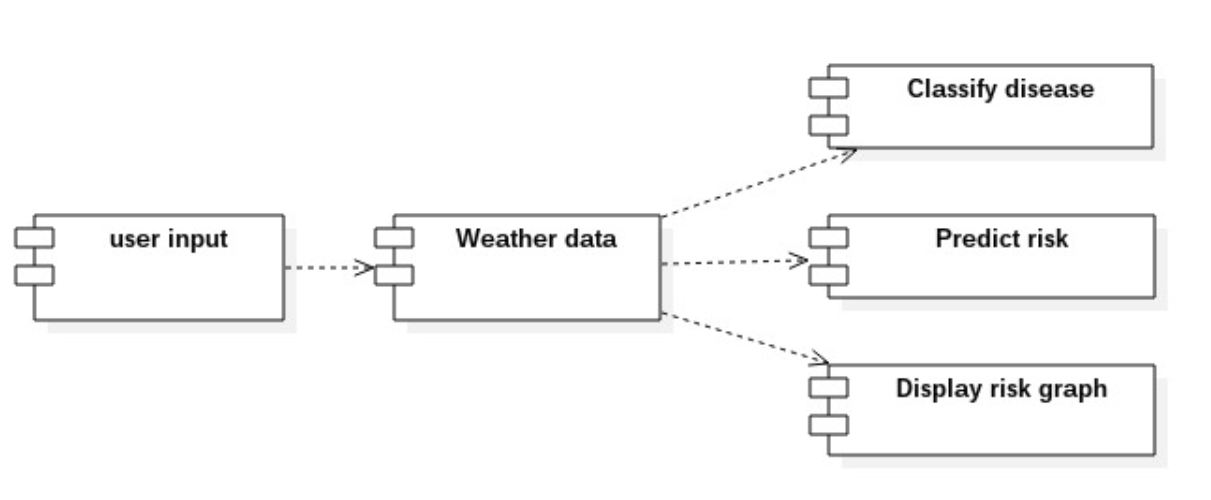
\includegraphics{3.png}}
		\caption{Use Case diagram-Connection}
	\end{center}
\end{figure}

\begin{figure}[!h]
	\begin{center}
		\scalebox{0.7}{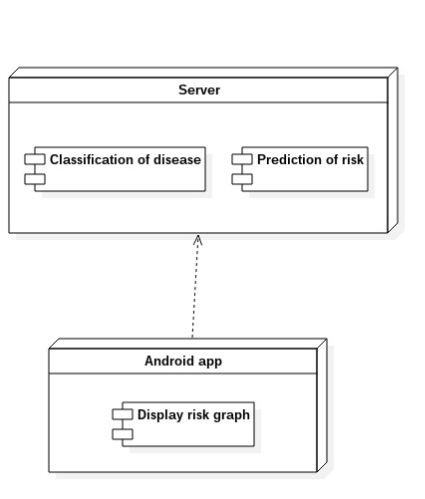
\includegraphics{4.png}}
		\caption{Use case diagram-Setting and Favouritism}
	\end{center}
\end{figure}

\begin{figure}[!h]
	\begin{center}
		\scalebox{0.7}{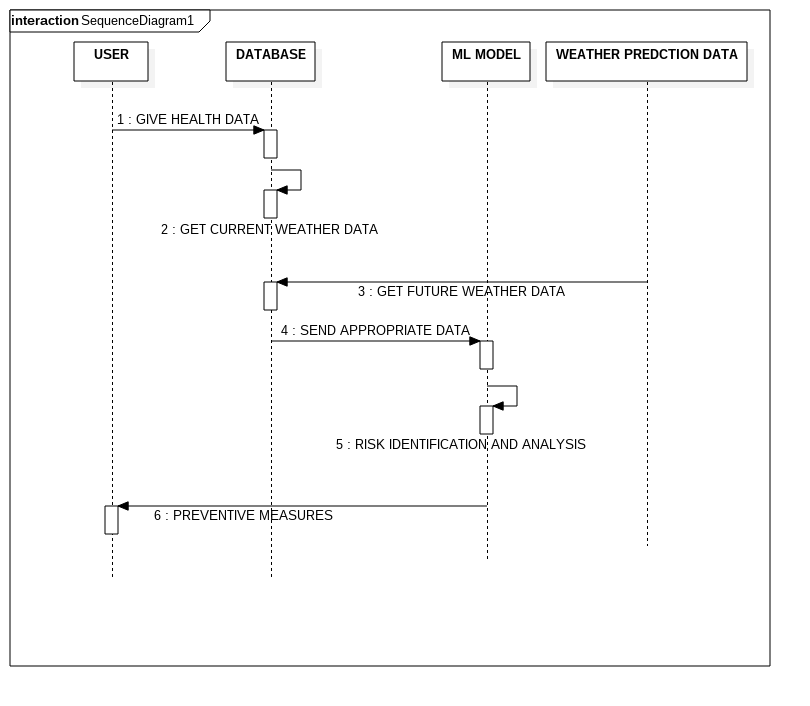
\includegraphics{5.png}}
		\caption{Use Case diagram-Working Device}
	\end{center}
\end{figure}


\newpage
\section{FUNCTIONAL MODEL AND DESCRIPTION}
\begin{enumerate}
\item \textbf{BluetoothAdapter}

The BluetoothAdapter is required for any and all Bluetooth activity. The BluetoothAdapter represents the device's own Bluetooth adapter (the Bluetooth radio). There's one Bluetooth adapter for the entire system, and your application can interact with it using this object. 

The first step in interacting with a BLE device is connecting to it— more specifically, connecting to the GATT server on the device. To connect to a GATT server on a BLE device, you use the connectGatt() method. This method takes three parameters: a Context object, autoConnect (boolean indicating whether to automatically connect to the BLE device as soon as it becomes available), and a reference to a BluetoothGattCallback
\item \textbf{onServicesDiscovered}

This function is called when the connection is established between the android phone and the Alerto device so as to know what further step is to be taken after connection.
\item \textbf{onCharacteristicRead}

The Alerto provides a ton of services which are read by the phone and services have various characteristics. The above function is used when the service and the characteristics of those services are explored and further step is to be decided.
\item Telephony manager

Provides access to information about the telephony services on the device. Applications can use the methods in this class to determine telephony services and states, as well as to access some types of subscriber information. Applications can also register a listener to receive notification of telephony state changes.
You do not instantiate this class directly; instead, you retrieve a reference to an instance through Context.getSystemService(Context.TELEPHONY\_SERVICE).
\end{enumerate}

 \subsection{Data Flow Diagram}
 \begin{itemize}
  \item{\textbf{Level 0 Data Flow Diagram}}
 \begin{figure}[!h]
 	\begin{center}
 		\scalebox{0.7}{\includegraphics{level0.png}}
 		\caption{Level 0 Data Flow Diagram}
 	\end{center}
 \end{figure}
 \newpage
 
 \item{\textbf{Level 1 Data Flow Diagram}}
\begin{figure}[!h]
	\begin{center}
		\scalebox{0.7}{\includegraphics{Level1.png}}
		\caption{Level 1 Data Flow Diagram}
	\end{center}
\end{figure}
\end{itemize}

\subsection{Activity Diagram}
In activity diagram the overall flow of the system is shown. It contains the following sequence of action.

\begin{figure}[h]
	\begin{center}
		\scalebox{1}{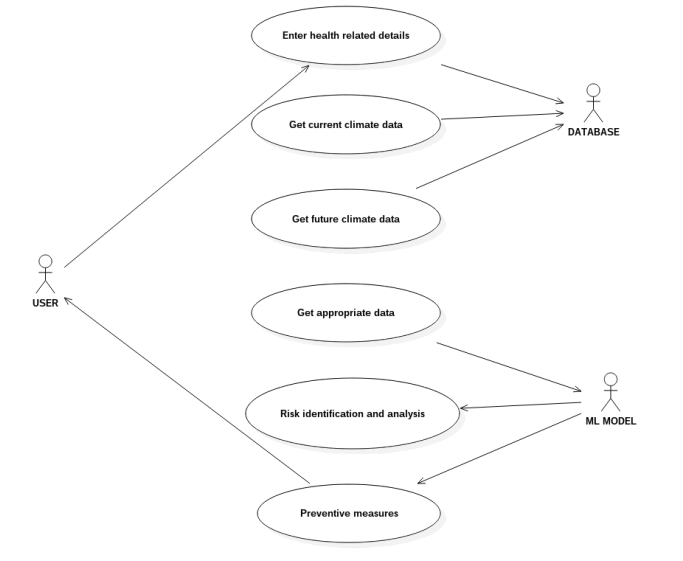
\includegraphics{1.png}}
		\caption{Activity diagram-Alerto Application}
	\end{center}
\end{figure}
\newpage
\begin{figure}[h]
	\begin{center}
		\scalebox{1}{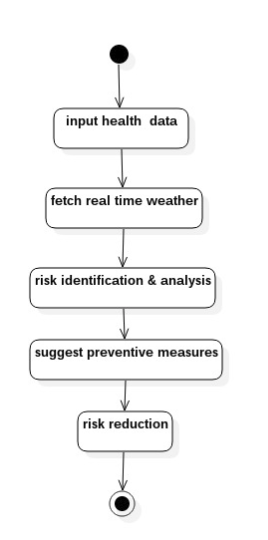
\includegraphics{2.png}}
		\caption{Activity diagram-User}
	\end{center}
\end{figure}

\subsection{Non Functional Requirements}

\begin{itemize}
	\item \textbf{Interface Requirements:}\\
Your app's user interface is everything that the user can see and interact with. Android provides a variety of pre-built UI components such as structured layout objects and UI controls that allow you to build the graphical user interface for your app. Android also provides other UI modules for special interfaces such as dialogs, notifications, and menus.

\item	\textbf{Performance Requirements:}
\begin{itemize}
\item Choosing the right algorithms and data structures should always be the priority. 
\item	do not allocate memory if you can avoid it
\item	To ensure your app performs well across a wide variety of devices, ensure your code is efficient at all levels and aggressively optimize your performance.\\
\end{itemize}
\begin{itemize}
\item	\textbf{Avoid Creating Unnecessary Objects}

Object creation is never free. A generational garbage collector with per-thread allocation pools for temporary objects can make allocation cheaper, but allocating memory is always more expensive than not allocating memory.

\item \textbf{Prefer Static Over Virtual}

If you do not need to access an object's fields, make your method static. Invocations will be about 15\%-20\% faster. It's also good practice, because you can tell from the method signature that calling the method can't alter the object's state.
\item \textbf{Consider Package Instead of Private Access with Private Inner Classes}
	
\end{itemize}
\item \textbf{Software quality attributes:}
	\begin{itemize}
		\item Availability
		
		\begin{itemize}
			\item It is the proportion of time a system is in a functioning condition.
			\item Availability of a system is typically measured as a factor of its reliability – as reliability increases, so does availability.
			\item Reliability needs to be evaluated and improved related to both availability and the cost of ownership (due to cost of spare parts, maintenance man-hours, transport costs, storage cost, part obsolete risks etc.).
			\item Fault tree analysis and related software are developed to calculate (analytic or by simulation) availability of a system or a functional failure condition within a system.
			\item In our case, our application is constantly available(running in the background).
		\end{itemize}
		\item Modifiability
		
		\begin{itemize}
			\item Portability
			
			\begin{itemize}
				\item Portability in high-level computer programming is the usability of the same software in different environments. The prerequirement for portability is the generalized abstraction between the application logic and system interfaces.
				\item Our application is not portable as it is supported only on android devices.
			\end{itemize}
			\item Reusability
			
			\begin{itemize}
				\item In computer science and software engineering, reusability is the use of existing assets in some form within the software product development process. Assets are products and by-products of the software development life cycle and include code, software components, test suites, designs and documentation.
				\item Subroutines or functions are the simplest form of reuse. A chunk of code is regularly organized using modules or namespaces into layers.
				\item The ‘vibration’ module in our code has been re-used for various types of incoming notifications.
			\end{itemize}
			\item Scalability
			
			\begin{itemize}
				\item An algorithm, design, networking protocol, program, or other system is said to scale if it is suitably efficient and practical when applied to large situations (e.g. a large input data set, a large number of outputs or users, or a large number of participating nodes in the case of a distributed system).
				\item We can scale our application to third party app notifications, such as WhatsApp, Emails, etc.
			\end{itemize}
		\end{itemize}
		\item Testability
		\begin{itemize}
			\item Software testability is the degree to which a software artifact (i.e. a software system, software module, requirements- or design document) supports testing in a given test context.
			\item It is an extrinsic property which results from interdependency of the software to be tested and the test goals, test methods used, and test resources (i.e., the test context).
			\item Our app is being tested for the following things:
			\begin{itemize}
				\item Connection of the Alerto with the android device.
				\item If the app is running even in the background.
				\item Vibration happening for following situations:
				\begin{enumerate}
					 	\item Arrival of notifications;
					 	\item Device going out of BLE range
					 	
				\end{enumerate}
				
			\end{itemize}
			
		\end{itemize}
		Note:  Detailed test cases have been provided in section 9.2.
		
		\item Usability
		\begin{itemize}
			\item In Software engineering, usability is the degree to which a software can be used by specified consumers to achieve quantified objectives with effectiveness, efficiency, and satisfaction in a quantified context of use.
			\item It includes methods of measuring usability, such as needs analysis and the study of the principles behind an object's perceived efficiency or elegance.
		    \item The primary notion of usability is:
			\begin{enumerate}
				 	\item More efficient to use, takes less time to accomplish a particular task
				 	\item Easier to learn—operation can be learned by observing the object
				 	\item More satisfying to use
				 	
				 	
			\end{enumerate}
		\end{itemize}
	\end{itemize}
\end{itemize}

\subsection{State Diagram}
State machine diagram capture the behavior of the software system. State machines can be used to model the behavior of a class or an entire application\\

\begin{figure}[!h]
	\begin{center}
		\scalebox{0.7}{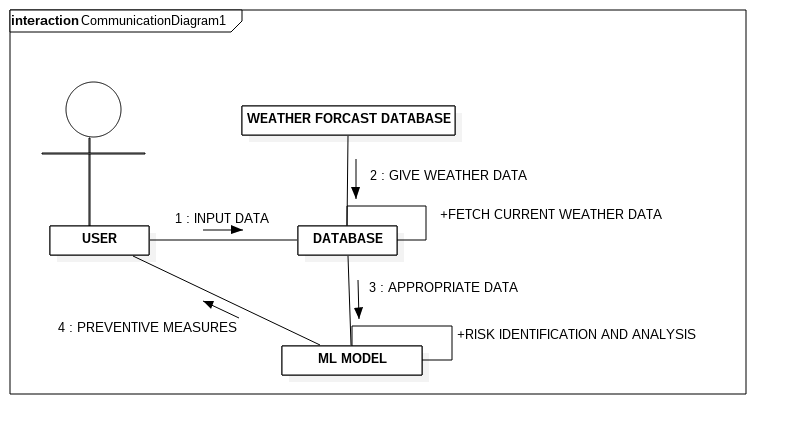
\includegraphics{6.png}}
		\caption{State Diagram}
	\end{center}
\end{figure}

\subsection{Design Constraints}
\begin{enumerate}
	\item	The android version used in the app should be higher than Jelly\_bean\_MR2(4.3+)
	\item	The distance between the Alerto device and Smartphone should be within Bluetooth LE range.
	\item	App requires access to contact details, Bluetooth information, Device ID and call information
	
\end{enumerate}

\subsection{Software Interface Description}
\begin{itemize}
	\item We are using android to provide an interface to the user.
	\item The software interface(Android) provides various options and buttons such as connection, selection of device, vibration patterns, disconnect which are used for interacting with the Alerto device.
	
\end{itemize}

\chapter{DETAILED DESIGN DOCUMENT USING APPENDIX A AND B}
\newpage

\section{INTRODUCTION}
\subsection{Purpose}
The purpose of this document is to describe the implementation of the Alerto Android Application. This app is designed to notify the user of his mobile calls \& notifications, when his phone isn't around him.
activities.
\subsection{Scope}
This document describes the implementation details of the Alerto Android Application. The app makes a Alerto device(wearable) vibrate, when being used by the user. It consists of major funcions such as: 
\begin{itemize}
\item	Connect- connects to the device; 
\item Send data- Vibration Patterns when any notification arrives.
\end{itemize}
\subsection{ Definitions, Acronyms, Abbreviations}
\subsubsection{Abbreviations}
\begin{itemize}
\item BLE: Bluetooth Low Energy
\item Android SDK: Android Software Development Kit
\end{itemize}

\subsubsection{Definitions}
\begin{itemize}
\item BLE: Compared to Classic Bluetooth, BLE is intended to provide considerably reduced power consumption and cost while maintaining a similar communication range.
\item Telephony Manager: A Java class(in Android) that provides access to information about the telephony services on the device. 
\item Broadcast Receiver: A broadcast receiver (short receiver) is an Android component which allows you to register for system or application events.
\item Services: A Service is an application component that can perform long-running operations in the background and does not provide a user interface.
\item Alerto Device: A wearable device that vibrates on phone's incoming notifications, when the phone's isn't with the person.
\end{itemize}

\section{ARCHITECTURAL DESIGN}
\begin{figure}[h]
	\begin{center}
		\scalebox{0.7}{\includegraphics{8.png}}
		\caption{Communication module using bluetooth LE}
	\end{center}
\end{figure}
\subsection{Bluetooth Low Energy:}

\hspace{0.5in}Compared to Classic Bluetooth, BLE is intended to provide considerably reduced power consumption and cost while maintaining a similar communication range. Mobile operating systems including iOS, Android, Windows Phone and BlackBerry, as well as OS X, Linux, and Windows 8, natively support BLE. BLE uses the same 2.4 GHz radio frequencies as Classic Bluetooth, which allows dual-mode devices to share a single radio antenna. LE does, however, use a simpler modulation system.\\\\
Internet Connectivity
\begin{itemize}
	\item IPSP (Internet Protocol Support Profile)
\end{itemize}
Generic Sensors
\begin{itemize}
	\item	ESP (Environmental Sensing Profile)
	\item	UDS (User Data Service)
\end{itemize}
HID Connectivity
\begin{itemize}
	\item HOGP (HID over GATT Profile)
\end{itemize}
Proximity sensing:

\hspace{0.5in}"Electronic leash" applications are well suited to the long battery life possible for 'always-on' devices.Manufacturers of iBeacon devices implement the appropriate specifications for their device to make use of proximity sensing capabilities supported by Apple Inc. compatible iDevices.\\\\
Relevant application profiles include:
\begin{itemize}
	\item FMP — the "find me" profile — allows one device to issue an alert on a second misplaced device.
	\item PXP — the proximity profile — allows a proximity monitor to detect whether a proximity reporter is within a close range. Physical proximity can be estimated using the radio receiver's RSSI value, although this does not have absolute calibration of distances. Typically, an alarm may be sounded when the distance between the devices exceeds a set threshold.
\end{itemize}
Alerts and time profiles
\begin{itemize}
	\item The phone alert status profile and alert notification profile allow a client device to receive notifications such as incoming call alerts from another device.
\end{itemize}

BLE has 40 2-MHz channels. Within a channel, data is transmitted using Gaussian frequency shift modulation, similar to Classic Bluetooth's Basic Rate scheme. The bit rate is 1Mbit/s, and the maximum transmit power is 10 mW. BLE uses frequency hopping to counteract narrow band interference problems. BLE is classified as a system using digital modulation techniques or a direct-sequence spread spectrum.

\begin{table}
	\caption{Bluetooth Vs Bluetooth Low Energy}
	\center
	\begin{tabular}{|p{4cm}|p{4cm}|p{4cm}|}
		\hline
		\textbf{Technical Specifications }& \textbf{Classic Bluetooth Technology} & \textbf{ Bluetooth Technology}\\
		\hline
		Distance/Range (theoretical max.) & 100 m (330 ft) & >100 m (>330 ft)\\
		\hline
		Over the air data rate & 1–3 Mbit/s	& 1 Mbit/s\\
		\hline
		Application throughput	& 0.7–2.1 Mbit/s & 0.27 Mbit/s\\
		\hline
		Active slaves	& 7	& Not defined; implementation dependent\\
		\hline
		Security	& 56/128-bit and application layer user defined & 128-bit AES with Counter Mode CBC-MAC and application layer user defined\\
		\hline
		Robustness	& Adaptive fast frequency hopping, FEC, fast ACK
		& Adaptive frequency hopping, Lazy Acknowledgement, 24-bit CRC, 32-bit Message Integrity Check\\
		\hline
		Latency (from a non-connected state) &	Typically 100 ms	& 6 ms\\
		\hline
		Minimum total time to send data (det.battery life)	& 100 ms &	3 ms \\
		\hline
		Voice capable &	Yes &	No\\
		\hline
		Network topology &	Scatternet & Scatternet\\
		\hline
		Power consumption	& 1 W as the reference	& 0.01 to 0.5 W (depending on use case)\\
		\hline
		Peak current consumption &	<30 mA &	<15 mA\\
		\hline
		Primary use cases &	Mobile phones, gaming, headsets, stereo audio streaming, smart homes, wearables, automotive, PCs, security, proximity, healthcare, sports and fitness, etc.	& Mobile phones, gaming, PCs, watches, sports and fitness, healthcare, security and proximity, automotive, home electronics, automation, Industrial, etc.\\
		\hline
	\end{tabular}
\end{table}

\newpage
\subsection{Bluetooth GATT(Software Model):}

All BLE devices use the Generic Attribute Profile (GATT). GATT has the following terminology:
\begin{itemize}
	\item Client:
	
	\hspace{0.5in}A device that initiates GATT commands and requests, and accepts responses, for example a computer or smartphone.
	\item Server:
	
	\hspace{0.5in} device that receives GATT commands and requests, and returns responses, for example a temperature sensor.
	\item Characteristic:
	
	\hspace{0.5in}A data value transferred between client and server, for example the current battery voltage.
	\item Service:
	
	\hspace{0.5in}A collection of related characteristics, which operate together to perform a particular function. Services may also include other services as sub-functions; the main functions of the device are so-called primaryservices, and the auxiliary functions they refer to are secondary services.
	\item Descriptor:
	
	\hspace{0.5in}A descriptor provides additional information about a characteristic. Descriptors are optional - each characteristic can have any number of descriptors.
	\item Identifier:
	
	\hspace{0.5in}Services, characteristics, and descriptors are collectively referred to as attributes, and identified by UUIDs. Any implementer may pick a random or pseudorandom UUID for proprietary uses, but the Bluetooth SIG have reserved a range of UUIDs (of the form xxxxxxxx-0000-1000-8000-00805F9B34FB ) for standard attributes. For efficiency, these identifiers are represented as 16-bit or 32-bit values in the protocol, rather than the 128 bits required for a full UUID. For example, the Device Information service has the short code 0x180A, rather than 0000180A-1000-….
	
	\item GATT Operation:
	
	\hspace{0.5in}The GATT protocol provides a number of commands for the client to discover information about the server. These include:
	\begin{itemize}
		\item 	Discover UUIDs for all primary services
		\item	Find a service with a given UUID
		\item	Find secondary services for a given primary service
		\item	Discover all characteristics for a given service
		\item	Find characteristics matching a given UUID
		\item	Read all descriptors for a particular characteristic.
	\end{itemize}
	
	Commands are also provided to read (data transfer from server to client) and write (from client to server) the values of characteristics:
	\begin{itemize}
		\item	A value may be read either by specifying the characteristic's UUID, or by a handle value (which is returned by the information discovery commands above).
		\item	Write operations always identify the characteristic by handle, but have a choice of whether or not a response from the server is required.
		\item	'Long read' and 'Long write' operations can be used when the length of the characteristic's data exceeds the MTU of the radio link.
	\end{itemize}
	
	Finally, GATT offers notifications and indications. The client may request a notification for a particular characteristic from the server. The server can then send the value to the client whenever it becomes available. An indication is similar to a notification, except that it requires a response from the client, as confirmation that it has received the message.
	\item  Battery impact:
	
	\hspace{0.5in}BLE is designed to enable devices with low power consumption. Devices with peripheral and central roles have different power requirements. A study by beacon software company. This is possible because of power efficiency of BLE protocol which only transmits small packets as compared to Bluetooth Classic which was also suitable for audio and high bandwidth data.
	In contrast, a continuous scan for the same beacons in central role can consume 1,000 mAh in few hours. With the newer chipsets and advances in software, both Android and iOS phones now have negligible power consumption in real-life BLE use scenarios.
\end{itemize}

\newpage
\begin{figure}[h]
	\begin{center}
		\scalebox{0.8}{\includegraphics{9.png}}
		\caption{Architecture Diagram}
	\end{center}
\end{figure}

\subsection{Services:}

A Service is an application component that can perform long-running operations in the background and does not provide a user interface. Another application component can start a service and it will continue to run in the background even if the user switches to another application. Additionally, a component can bind to a service to interact with it and even perform interprocess communication (IPC). 
A service can essentially take two forms:
\begin{itemize}
	\item \textbf{Started:}
	
	\hspace{0.5in}A service is "started" when an application component (such as an activity) starts it by calling startService(). Once started, a service can run in the background indefinitely, even if the component that started it is destroyed. Usually, a started service performs a single operation and does not return a result to the caller. For example, it might download or upload a file over the network. When the operation is done, the service should stop itself.
	\item \textbf{Bound:}
	
	\hspace{0.5in}A service is "bound" when an application component binds to it by calling bindService(). A bound service offers a client-server interface that allows components to interact with the service, send requests, get results, and even do so across processes with interprocess communication (IPC). A bound service runs only as long as another application component is bound to it. Multiple components can bind to the service at once, but when all of them unbind, the service is destroyed.
	
\end{itemize}

\subsection{Activities :}
An Activity is an application component that provides a screen with which users can interact in order to do something, such as dial the phone, take a photo, send an email, or view a map. Each activity is given a window in which to draw its user interface. The window typically fills the screen, but may be smaller than the screen and float on top of other windows.

An application usually consists of multiple activities that are loosely bound to each other. Typically, one activity in an application is specified as the "main" activity, which is presented to the user when launching the application for the first time. Each activity can then start another activity in order to perform different actions. Each time a new activity starts, the previous activity is stopped, but the system preserves the activity in a stack (the "back stack"). When a new activity starts, it is pushed onto the back stack and takes user focus. The back stack abides to the basic "last in, first out" stack mechanism, so, when the user is done with the current activity and presses the Back button, it is popped from the stack (and destroyed) and the previous activity resumes. 

When an activity is stopped because a new activity starts, it is notified of this change in state through the activity's lifecycle callback methods. There are several callback methods that an activity might receive, due to a change in its state—whether the system is creating it, stopping it, resuming it, or destroying it—and each callback provides you the opportunity to perform specific work that's appropriate to that state change. For instance, when stopped, your activity should release any large objects, such as network or database connections. When the activity resumes, you can reacquire the necessary resources and resume actions that were interrupted. These state transitions are all part of the activity lifecycle.

.

\subsection{Telephony Manager :}
Provides access to information about the telephony services on the device. Applications can use the methods in this class to determine telephony services and states, as well as to access some types of subscriber information. Applications can also register a listener to receive notification of telephony state changes.
You do not instantiate this class directly; instead, you retrieve a reference to an instance throughContext.getSystemService(Context.TELEPHONY\_SERVICE).

Note that access to some telephony information is permission-protected. Your application cannot access the protected information unless it has the appropriate permissions declared in its manifest file. Where permissions apply, they are noted in the the methods through which you access the protected information.


\subsection{Broadcast Manager:}	
Helper to register for and send broadcasts of Intents to local objects within your process. This is has a number of advantages over sending global broadcasts with sendBroadcast(Intent): 
\begin{itemize}
	\item	You know that the data you are broadcasting won't leave your app, so do not need to worry about leaking private data. 
	\item	It is not possible for other applications to send these broadcasts to your app, so you do not need to worry about having security holes they can exploit. 
	\item	It is more efficient than sending a global broadcast through the system. 
\end{itemize}

\section{COMPONENT DESIGN}
\begin{itemize}
\item Component-level design occurs after the first iteration of the architectural design
\item It strives to create a design model from the analysis and architectural models
\begin{itemize}
\item The translation can open the door to subtle errors that are difficult to find and correct later
\item "Effective programmers should not waste their time debugging – they should not introduce bugs to start with."  Edsgar Dijkstra
\end{itemize}
\item A component-level design can be represented using some intermediate representation (e.g. graphical, tabular, or text-based) that can be translated into source code
\item The design of data structures, interfaces, and algorithms should conform to well-established guidelines to help us avoid the introduction of errors
\end{itemize}

\subsection{Class Diagram}
Class diagram are the most common diagram found in modeling object oriented systems. A class diagram shows set of classes interface and collaboration and their relationships.
\begin{figure}[h]
	\begin{center}
		\scalebox{0.8}{\includegraphics{11.png}}
		\caption{Class Diagram}
	\end{center}
\end{figure}

\chapter{PROJECT IMPLEMENTATION}
\newpage

\section{INTRODUCTION}
Our project is a simple application.We are using android for implementation of our project. We have implemented on Android SDK which uses java and xml languages. Our app is using the Bluetooth LE technology which is much more cost effective than Bluetooth and has a greater battery life.

While implementing we have used classes and module based implementation is done. 

\section{TOOLS AND TECHNOLOGIES USED}
\subsection{HARDWARE RESOURCES }
\begin{enumerate}
	\item	400MB Hard disk+1GB for Android SDK, emmulator system images and caches
	\item	Alerto device(Wearable)
	\item	2GB RAM minimum,4GB RAM recommended
	\item	Intel Processor with support for Intel VT-x, Intel EM64T(Intel 64)
	\item	Computer  with windows Vista/7/8.
	
\end{enumerate}

\subsection{SOFTWARE RESOURCES }

\begin{itemize}
	\item Platform: Android SDK
	\item  Operating System: Android
	\item  Programming Language: Java, XML.
\end{itemize}

\subsection{TECHNOLOGY}
\begin{itemize}
	\item Bluetooth LE
\end{itemize}

\section{METHOLOGIES AND ALGORITHMS DETAILS}
\subsection{Algorithm For Bluetooth LE Connecttion Establishment}
\begin{enumerate}
	\item Bluetooth is turned on.
	\item Beacons are broadcasted for connection.
	\item Device requests for connection. 
	\item User needs to select the device and press connect.
	\item Connection completed.
\end{enumerate}
\subsection{Algorithm For Execution of the Android App}
\begin{enumerate}
	\item Install the app on android phone.
	\item Turn on phone's bluetooth and select the device for connection. 
	\item The app is running in background in the phone.If:
	Incoming notification received-send vibrate() command to Alerto device.
	\item Device vibrates
\end{enumerate}

\section{VERIFICATION AND VALIDATION FOR ACCEPTANCE}
\hspace{0.2 in}In software project management, software testing, and software engineering, verification and validation (V\&V) is the process of checking that a software system meets specifications and that it fulfills its intended purpose. It may also be referred to as software quality control. It is normally the responsibility of software testers as part of the software development lifecycle.

\hspace{0.2 in}Validation checks that the product design satisfies or fits the intended use (high-level checking), i.e., the software meets the user requirements. This is done through dynamic testing and other forms of review.

\hspace{0.2 in}Verification and validation are not the same thing, although they are often confused. Boehmsuccinctly expressed the difference between
\begin{itemize}
	\item Verification: Are we building the product right?
	\item Validation: Are we building the right product?
\end{itemize}

\hspace{0.2 in}According to the Capability Maturity Model 
\begin{itemize}
	\item Software Verification: The process of evaluating software to determine whether the products of a given development phase satisfy the conditions imposed at the start of that phase. 
	\item Software Validation: The process of evaluating software during or at the end of the development process to determine whether it satisfies specified requirements.
\end{itemize}

\hspace{0.2 in}Verification: In our project we have compared and used various technologies which will be best fit for the application
\begin{enumerate}
	\item Our project is based on Android operating system but it can be implemented on other operating systems as well. However we have selected Android because it is much more popular in comparison to other OSs which increases the usability of our application.
	\item Bluetooth Low energy uses less amount of battery power as compared to regular Bluetooth devices. Hence using this technology helps to reduce power consumption and increase battery life. Thus we have used this technology for our application
\end{enumerate}

\chapter{SOFTWARE TESTING}
\newpage

\section{TYPES OF TESTING USED}
\hspace{0.2 in}Since our application is on android, we have done manual testing.There are different stages for manual testing such as unit testing, integration testing,system testing, and user acceptance testing.
\begin{enumerate}
	\item \textbf{Unit testing}
	
	\hspace{0.2 in}In computer programming, unit testing is a software testing method by which individual units of source code, sets of one or more computer program modules together with associated control data, usage procedures, and operating procedures, are tested to determine whether they are fit for use.
	
	\hspace{0.2 in}In our program, we have units such as Connection() which is used for connection, Vibrate() to check if the vibration occurs, and different modules for checking if device vibrates when incoming call, Incoming message or notification from third party app comes on the android phone which have been successfully tested unitwise.
	\item \textbf{Integration testing}
	
	\hspace{0.2 in}Integration testing (sometimes called integration and testing, abbreviated I\&T) is the phase in software testing in which individual software modules are combined and testedas a group. It occurs after unit testing and before validation testing.
	
	\hspace{0.2 in}In our program we have integrated the connection and vibration module to be tested as integration testing. Also we have integrated the modules which the functionality of vibration for different incoming notifications.
	\item \textbf{System testing}
	
	\hspace{0.2 in}System testing of software or hardware is testing conducted on a complete, integrated system to evaluate the system's compliance with its specified requirements. System testing falls within the scope of black-box testing, and as such, should require no knowledge of the inner design of the code or logic.
	\hspace{0.2 in}We have successfully performed the system testing in which the system was tested as a whole.
	\item \textbf{User Acceptance testing}
	
	\hspace{0.2 in}User acceptance testing (UAT) is the last phase of the softwaretesting process. During UAT, actual software users test the software to make sure it can handle required tasks in real-world scenarios, according to specifications. We have successfully completed this testing.
\end{enumerate}

\section{TEST CASES AND TEST RESULTS}

\begin{table}[!h]

		\begin{tabular}{|p{0.8cm}|p{2.5cm}|p{3cm}|p{3cm}|p{3cm}|p{2.2cm}|}
			\hline
			\multicolumn{6}{|l|}{Project Name:Alerto}\\
			\hline
			\multicolumn{6}{|l|}{Test Case ID:001}\\
			\hline
			\multicolumn{6}{|l|}{Test Priority(Low/Med/High):High} \\ 
			\hline
			\multicolumn{6}{|l|}{Test Designed and Executed by:Student}\\
			\hline
			\multicolumn{6}{|l|}{Test Designed and Executed date:01/04/2016}\\
			\hline
			\multicolumn{6}{|l|}{Module Name:Connection} \\ 
			\hline
			\multicolumn{6}{|l|}{Test Title:Testcase1} \\
			\hline
			\multicolumn{6}{|l|}{Description:Checking if the device(Alerto) and Android phone connect} \\
			\hline
			 \\
			\hline
			\multicolumn{6}{|l|}{Pre-conditions: Show the connection UI to user.}\\
			\hline
			\multicolumn{6}{|l|}{Post condition: The Alerto device and android phone connect over Bluetooth  low energy.}\\
			\hline
			Steps & Test steps & Test data & Expected Result & Actual Result & Status \\ 
			\hline
			1	& Check whether the application gets started.& 	Running the application	& The app starts when run.&	The app starts when run. &	pass\\ 
			\hline
			2&	Check if available devices for connection are shown.&	Available devices information	& All devices in range are shown&	All device in range are shown	& pass\\
			\hline
			3&	Check if the selected device gets connected.&	Selected device.&	Successful connection and device information &	Successful connection and device information	& pass \\
			\hline
			4 &	Check if connection occurs when device is out of range.&	Out of range device &	Shows error message. &	Abruptly disconnects &	fail \\
			\hline
		\end{tabular}
\end{table}

\begin{table}[!h]
	
	\begin{tabular}{|p{0.8cm}|p{2.5cm}|p{3cm}|p{3cm}|p{3cm}|p{2.2cm}|}
		\hline
		\multicolumn{6}{|l|}{Project Name:Alerto}\\
		\hline
		\multicolumn{6}{|l|}{Test Case ID:002}\\
		\hline
		\multicolumn{6}{|l|}{Test Priority(Low/Med/High):High} \\ 
		\hline
		\multicolumn{6}{|l|}{Test Designed and Executed by:Student}\\
		\hline
		\multicolumn{6}{|l|}{Test Designed and Executed date:01/04/2016}\\
		\hline
		\multicolumn{6}{|l|}{Module Name:Vibration} \\ 
		\hline
		\multicolumn{6}{|l|}{Test Title:Testcase2} \\
		\hline
		\multicolumn{6}{|l|}{Description:Check if after connection, device vibrates on pressing vibrate button.}\\
		\hline
		\\
		\hline
		\multicolumn{6}{|l|}{Pre-conditions: Show the vibration UI to user.}\\
		\hline
		\multicolumn{6}{|l|}{Post condition: : Device vibrates after giving the command.}\\
		\hline
		Steps & Test steps & Test data & Expected Result & Actual Result & Status \\ 
		\hline
		1	& Check whether vibrate key is working correctly.	& Vibration Byte data.&	Key should work correctly.	& Key is working correctly.& Pass\\
		\hline
		2	& Check if vibration occurs.	& Byte data.&	Device should vibrate.&	Device is vibrating after giving command.&	Pass\\
		\hline
	\end{tabular}
\end{table}

\begin{table}[!h]
	
	\begin{tabular}{|p{0.8cm}|p{2.5cm}|p{3cm}|p{3cm}|p{3cm}|p{2.2cm}|}
		\hline
		\multicolumn{6}{|l|}{Project Name:Alerto}\\
		\hline
		\multicolumn{6}{|l|}{Test Case ID:003}\\
		\hline
		\multicolumn{6}{|l|}{Test Priority(Low/Med/High):High} \\ 
		\hline
		\multicolumn{6}{|l|}{Test Designed and Executed by:Student}\\
		\hline
		\multicolumn{6}{|l|}{Test Designed and Executed date:01/04/2016}\\
		\hline
		\multicolumn{6}{|l|}{Module Name:Call} \\ 
		\hline
		\multicolumn{6}{|l|}{Test Title:Testcase3} \\
		\hline
		\multicolumn{6}{|l|}{Description:: Checking if device vibrates when call comes} \\
		\hline
		\\
		\hline
		\multicolumn{6}{|l|}{Pre-conditions: App running.}\\
		\hline
		\multicolumn{6}{|l|}{Post condition: Alerto device vibrates when notification of call comes on phone..}\\
		\hline
		Steps & Test steps & Test data & Expected Result & Actual Result & Status \\ 
		\hline
		1&	Check whether device vibrates.&	Notification from call.&	Device vibrates on notification.&	Device vibrates on notification.&	Pass\\
		\hline
		2&	Check if device vibrated when out of range.&	Notification from call.&	Error message.&	Device disconnected.&	Fail\\
		
		\hline
	\end{tabular}
\end{table}

\begin{table}[!h]
	
	\begin{tabular}{|p{0.8cm}|p{2.5cm}|p{3cm}|p{3cm}|p{3cm}|p{2.2cm}|}
		\hline
		\multicolumn{6}{|l|}{Project Name:Alerto}\\
		\hline
		\multicolumn{6}{|l|}{Test Case ID:004}\\
		\hline
		\multicolumn{6}{|l|}{Test Priority(Low/Med/High):High} \\ 
		\hline
		\multicolumn{6}{|l|}{Test Designed and Executed by:Student}\\
		\hline
		\multicolumn{6}{|l|}{Test Designed and Executed date:01/04/2016}\\
		\hline
		\multicolumn{6}{|l|}{Module Name:Messages} \\ 
		\hline
		\multicolumn{6}{|l|}{Test Title:Testcase4} \\
		\hline
		\multicolumn{6}{|l|}{Description:: Checking if device vibrates when nessages comes} \\
		\hline
		\\
		\hline
		\multicolumn{6}{|l|}{Pre-conditions: App running.}\\
		\hline
		\multicolumn{6}{|l|}{Post condition: Alerto device vibrates when message comes on phone..}\\
		\hline
		Steps & Test steps & Test data & Expected Result & Actual Result & Status \\ 
		\hline
		1&	Check whether device vibrates.&	Notification from messages.&	Device vibrates on notification.&	Device vibrates on notification.&	Pass\\
		\hline
		2&	Check if device vibrated when out of range.&	Notification from messages.&	Error message.&	Device disconnected.&	Fail\\
		
		\hline
	\end{tabular}
\end{table}

\begin{table}[!h]
	
	\begin{tabular}{|p{0.8cm}|p{2.5cm}|p{3cm}|p{3cm}|p{3cm}|p{2.2cm}|}
		\hline
		\multicolumn{6}{|l|}{Project Name:Alerto}\\
		\hline
		\multicolumn{6}{|l|}{Test Case ID:005}\\
		\hline
		\multicolumn{6}{|l|}{Test Priority(Low/Med/High):High} \\ 
		\hline
		\multicolumn{6}{|l|}{Test Designed and Executed by:Student}\\
		\hline
		\multicolumn{6}{|l|}{Test Designed and Executed date:01/04/2016}\\
		\hline
		\multicolumn{6}{|l|}{Module Name:NotificationListenersService} \\ 
		\hline
		\multicolumn{6}{|l|}{Test Title:Testcase5} \\
		\hline
		\multicolumn{6}{|l|}{Description:: Checking if device vibrates when third party apps give notification} \\
		\hline
		\\
		\hline
		\multicolumn{6}{|l|}{Pre-conditions: App running.}\\
		\hline
		\multicolumn{6}{|l|}{Post condition: Alerto device vibrates when notification of third party apps comes on phone..}\\
		\hline
		Steps & Test steps & Test data & Expected Result & Actual Result & Status \\ 
		\hline
		1&	Check whether device vibrates.&	Notification from third party apps.&	Device vibrates on notification.&	Device vibrates on notification.&	Pass\\
		\hline
		2&	Check if device vibrated when out of range.&	Notification from third party apps.&	Error message.&	Device disconnected.&	Fail\\
		
		\hline
	\end{tabular}
\end{table}

\chapter{RESULTS}
\newpage

\section{SCREEN SHOTS}
	\begin{figure}[!h]
		\begin{center}
			\scalebox{0.15}{\includegraphics{14 (1).png}}
		\end{center}
	\end{figure}
	
		\begin{figure}[!h]
			\begin{center}
				\scalebox{0.15}{\includegraphics{14 (2).png}}
			\end{center}
		\end{figure}
				\begin{figure}[!h]
				\begin{center}
					\scalebox{0.15}{\includegraphics{14 (3).png}}
				\end{center}
			\end{figure}
				\begin{figure}[!h]
					\begin{center}
				\scalebox{0.15}{\includegraphics{14 (4).png}}
					\end{center}
				\end{figure}
					\begin{figure}[!h]
						\begin{center}
							\scalebox{0.15}{\includegraphics{14 (5).png}}
						\end{center}
					\end{figure}
					
\chapter{DEPLOYMENT AND MAINTENANCE}
\newpage

\section{INSTALLATION AND UN-INSTALLATION}
\subsection{Installation}
Once we execute the application it gets installed on the phone automatically. The Alerto device is connected to the phone via Bluetooth low energy. When an incoming call or message is received on the phone,  the Alerto will vibrate informing the user about the notification. When we stop the execution of the code,  the app remains installed on Android phone
\subsection{Un-installation}
The app needs to be manually removed from the phone as it exist even after we stop running the code.

\section{USER HELP}
Our app is quite simple.We have made it very user-friendly.The user can  easily navigate through the pages of the app.

\chapter{\bf{FUTURE ENHANCEMENT AND CONCLUSION}}
\newpage

\section{FUTURE SCOPE}
In the future,we want to add the following as enhancement:
\begin{enumerate}
	\item The favouritism can be extended to emails.
	\item The application can be used with other wearable devices also, which are using bluetooth LE technology.
	 \item Further more options for alarms can be added to the application.
\end{enumerate}

\section{CONCLUSION}
\hspace{0.5in}In ths project we are developing a mobile based "Alerto" application. This application would help to notify the user whenever a notification arrives on its phone.\\\\
The system uses bluetooth low energy technology which is used to sync our mobile devices with a wearable device called "Alerto". Whenever a notification arrives on our mobile phone the Alerto notifies the user with a vibration.\\

Thus, we successfully solved the problem of being worried for an important phone call because this application separates the messages/calls from the important ones.\\

In future, more functionalities can be added to use this application with another device with more features.With the advent of smart phones,when developed to its fullest would be able for all to use.


\chapter{REFERENCES}
\newpage

\bibliographystyle{ieeetr} 

\begin{thebibliography}{1}
\addcontentsline{toc}{chapter}{BIBLIOGRAPHY}
\bibitem{IEEEhowto:Wu} Jia Liu, Member, IEEE, Canfeng Chen, Member, IEEE, and Yan Ma, Member, IEEE\\ Modeling Neighbor Discovery in Bluetooth Low Energy Networks\\ 
IEEE COMMUNICATIONS LETTERS, VOL. 16, NO. 9, SEPTEMBER 2012
\bibitem{IEEEhowto:Wu}Jia Liu, Member, IEEE, Canfeng Chen, Member, IEEE, and Yan Ma, Member, IEEE\\ Energy Analysis of Device Discovery for
	Bluetooth Low Energy, 2013

\bibitem{IEEEhowto:Wu}	Jia Liu, Member, IEEE, Canfeng Chen, Member, IEEE, and Yan Ma, Member, IEEE\\ Advertising semantically described physical items
	with Bluetooth Low Energy beacons, 2013\\
	2nd Mediterranean Conference on Embedded Computing ,,/" MECD - 2013
\bibitem{IEEEhowto:Wu}
Takeshi Iwamoto1, Nobuhiko Nishio1, and Hideyuki Tokuda1,2\\ Wapplet: A Media Access Framework for
	Wearable Applications, 2002\\
	1. Graduate School of Media and Governance, Keio University, Japan
	{iwaiwa, vino, hxt}@ht.sfc.keio.ac.jp\\
	2.Faculty of Environmental Information, Keio University, Japan
\bibitem{IEEEhowto:Wu} 	Anindya Nag and Subhas Chandra Mukhopadhyay\\
Wearable Electronics Sensors: Current Status
	and Future Opportunities, 2015\\
	Massey University,
	Palmerston North, New Zealand 
\end{thebibliography}

\begin{appendices}
\chapter{LABORATORY ASSIGNMENTS ON PROJECT ANALYSIS OF ALGORITHM DESIGN}
\newpage

\begin{itemize}
	\item To develop the problem under consideration and justify feasibilty using
	concepts of knowledge canvas and IDEA Matrix.
	
	\hspace{0.5in}IDEA Matrix is represented in the following form. Knowledge canvas represents about identification of opportunity for product. Feasibility is represented w.r.t. business perspective.
	\begin{table}[!h]
		\centering
		\begin{tabular}{|p{2cm}|p{2cm}|p{2cm}|p{2cm}|}
		\hline
			I & D & E & A\\
			\hline
			Increase & Drive & Educate & Accelerate\\
			\hline
			Improve& Deliver& Evaluate& Associate\\
			\hline
			Ignore& Decrease& Eliminate& Avoid\\
			\hline
		\end{tabular}
		\caption{IDEA Matrix}
	\end{table}
	
	\item Project problem statement feasibility assessment using NP-Hard, NP-
	Complete or satisfy ability issues using modern algebra and/or relevant
	mathematical models.
	
	\textbf{Polynomial(P) and Non-Polynomial(NP)}
	\begin{itemize}
\item 	Polynomial Time:\\
	\hspace{0.5in}The class of polynomial- time solvable problems P includes all the sets in which membership may be decided by an algorithm whose running time is bounded by a polynomial.\\
	Example:
	\begin{itemize}
	\item Linear Time-O(n)
	\item Quadratic Time-O(n2)
	\item Exponential Time-O(2n)
	\item Logarithmic Time-O(logn)
	\end{itemize}
	
	\item Non-Polynomial Time:\\
	\hspace{0.5in}The class non-deterministic polynomially acceptable problems, NP contains all sets in which membership can be verified in polynomial time. All problems from P is also NP.
	Examples:
	\begin{itemize}
	\item Decision problem version of the integer factorisation problem
	\item Graph isomorphism problem
	\item A decision version of travelling salesman problem
	\item The Boolean satisfiability problem\\
		\end{itemize}
		
		Types of NP type problems:
		\begin{itemize}
		\item NP-hard:\\
	\hspace{0.5in}In computational complexity theory, is a class of problems that are, informally, "at least as hard as the hardest problems in NP". More precisely, a problem H is NP-hard when every problem L in NP can be reduced in polynomial time to H.As a consequence, finding a polynomial algorithm to solve any NP-hard problem would give polynomial algorithms for all the problems in NP, which is unlikely as many of them are considered hard.
	
	\item NP-complete:\\
	\hspace{0.5in}In computational complexity theory, a decision problem is NP-complete when it is both in NP and NP-hard. The set of NP-complete problems is often denoted by NP-C or NPC. The abbreviation NP refers to "nondeterministic polynomial time".\\
\end{itemize}
	\hspace{0.5in}Thus from the above definition our application of is P (Polynomial) class.
\end{itemize}
\item \textbf{Input x,Output y, y=f(x)}
\begin{itemize}
	

\item I:Set of Inputs=\{I1, I2\}\\
where,
\begin{itemize}
\item I1: Installation of the Android application ‘Alerto’
\item I2: Running of the application
\end{itemize}
\item O: Set of Outputs=\{O1, O2\}\\
where,
\begin{itemize}
\item O1: List of available Alertos
\item O2: Connection established with a particular Alerto.
\end{itemize}
\item F:Set of Functions=\{F1, F2, F3, F4, F5\}\\
where,
\begin{itemize}
\item F1: Get started with the application.
\item F2: Turn on Bluetooth.
\item F3: Scan for available Alerto devices in range.
\item F4: Connect with specific Alerto.
\item F5: Once desired notification arrives on emulator, the particular Alerto vibrates.
\end{itemize}
\end{itemize}
\end{itemize}

\chapter{LABORATORY ASSIGNMENTS ON PROJECT QUALITY AND RELIABILITY TESTING OF PROJECT DESIGN}
\newpage

\begin{itemize}
	\item Use of divide and conquer strategies to exploit distributed/parallel/concurrent processing of the above to identify object, morphisms, overloading in functions (if any), and functional relations and any other dependencies (as per requirements). It can include Venn diagram, state diagram, function relations, i/o relations; use this to derive objects, morphism,
	overloading\\
	\hspace{0.5 in}With this strategy, a problem is solved by splitting it into sub-problems, solving them independently, and merging their solutions into a solution for the whole problem. The sub-problems can be solved directly, or they can in turn be solved using the same divide-and-conquer strategy, leading to an overall recursive program structure. The potential concurrency in this strategy is not hard to see: Since the sub-problems are solved independently, their solutions can be computed concurrently, leading to a parallel program that is very similar to its sequential counterpart. The following figure illustrates the strategy and the potential concurrency.
	\begin{figure}[!h]
		\begin{center}
		\scalebox{0.7}{\includegraphics{DividenConquers.png}}
		\caption{Divide and Conquer Strategy}
		\end{center}
	\end{figure}
	\textbf{Identify Morphism}\\
	\hspace{0.5 in}Much of the terminology of morphisms, as well as the intuition underlying them, comes from concrete categories, where the objects are simply sets with some additional structure, and morphisms are structure-preserving functions.
	\hspace{0.5 in}A category C consists of two classes, one of objects and the other of morphisms.
	There are two objects that are associated to everymorphism, the source and the target.
	\hspace{0.5 in}For many common categories, objects are sets (usually with more structure) and morphisms are functions from an object to another object. Therefore the source and the target of a morphism are often called respectively domain and codomain.
	\hspace{0.5 in}A morphism f with source X and target Y is written f : X → Y. Thus a morphism is represented by an arrow from its source to its target.
	In the category of smooth manifolds, morphisms are smooth functions and isomorphisms are called diffeomorphisms.
	
	\textbf{Functional Dependency}\\
	\hspace{0.5 in}Functional dependency is a relationship that exists when one attribute uniquely determines another attribute.
	\hspace{0.5 in}If R is a relation with attributes X and Y, a functional dependency between the attributes is represented as X->Y, which specifies Y is functionally dependent on X. Here X is a determinant set and Y is a dependent attribute. Each value of X is associated precisely with one Y value.
	
	
	\item Use of above to draw functional dependency graphs and relevant Software modeling methods, techniques including UML diagrams or other
	necessities using appropriate tools.
	\begin{enumerate}
		\item To draw functional dependency graph.
		\begin{figure}[!h]
			\begin{center}
				\scalebox{0.7}{\includegraphics{functndep.png}}
				\caption{Functional Dependency Graph}
			\end{center}
		\end{figure}
			\newpage
		\item UML diagrams or other necessities using appropriate tools.
		UML diagrams consists of following diagrams:
		\begin{enumerate}
			\item Use-Case Diagram
			\item Activity Diagram
			\item State Diagram
			\item Component Diagram
			\item Class Diagram
			\item Package Component Diagram
			\item Deployment Diagram
			\item Sequence Diagram
			
		\end{enumerate}
	\end{enumerate}

	\item Testing of project problem statement using generated test data (using
	mathematical models, GUI, Function testing principles, if any) selection and appropriate use of testing tools, testing of UML diagram's
	reliability. Write also test cases [Black box testing] for each identified
	functions. You can use Mathematica or equivalent open source tool for generating test data.\\
	\hspace{0.5 in}Software testing can be stated as process of validating and verifying that a computer program/application/product:
	\begin{itemize}
		\item Meets the requirements that guided its design and development.
		\item Works as expected.
		\item Can be implemented with the same characteristics.
		\item Satisfies the needs of stake holders.
		
	\end{itemize}
	
	\hspace{0.5 in}Software testing, depending on the testing methods employed, can be implemented at any time in the development process. Traditionally, most of the test efforts occur after the requirements have been defined and the coding process has been completed but in the agile approaches most of the test effort is ongoing. As such the methodology of test is governed by a chosen software development methodology.
	
	\textbf{Types of testing:}
	\begin{itemize}
		\item \textbf{Unit testing:}\\
		Unit testing is a software testing method by which individual units of source code, sets of one or more computer program modules together with associated control data, usage procedures, and operating procedures, are tested to determine whether they are fit for use. Intuitively, one can view a unit as the smallest testable part of an application. In procedural programming, a unit could be an entire module, but it is more commonly an individual function or procedure. In object-oriented programming, a unit is often an entire interface, such as a class, but could be an individual method. Unit tests are short code fragments created by programmers or occasionally by white box testers during the development process. It forms the basis for component testing. 
		\item \textbf{Integration testing:}\\
		Integration testing is the phase in software testing in which individual software modules are combined and tested as a group. It occurs after unit testing and before validation testing. Integration testing takes as its input modules that have been unit tested, groups them in larger aggregates, applies tests defined in an integration test plan to those aggregates, and delivers as its output the integrated system ready for system testing.
		\item \textbf{Acceptance testing:}\\
		Acceptance testing is a test conducted to determine if the requirements of a specification or contract are met. It may involve chemical tests, physical tests, or performance tests.
		In systems engineering it may involve black-box testing performed on a system (for example: a piece of software, lots of manufactured mechanical parts, or batches of chemical products) prior to its delivery. 
		
	\end{itemize}
	
	\textbf{Test Cases}
	\begin{enumerate}
		\item List of devices shown properly.
		\item Connection established.
		\item Configuration of Settings.
		\item Notifications alerted.
		\item Correct notifications are alerted
		
	\end{enumerate}
	
	\textbf{GUI testing}\\
	\hspace{0.5 in}GUI test is for testing if the GUI we have made for the application is working in the correct manner as desired. In our application we are going to have many buttons and lists so we will be checking if they are working properly.
	
\end{itemize}

\chapter{PROJECT PLANNER}
\newpage


\begin{table}[h]
	
	\caption {Plan of Project}
	\center
	\begin{tabular}{ |p{3cm}|p{3cm}|p{3cm}|p{3cm}|  }
		
		\hline
		From & To & Task & Status\\
		\hline
		27\textendash06\textendash2015 & 30\textendash06\textendash2015 & Group Formation and finalization &  Done\\
		\hline
		
		01\textendash07\textendash2015 & 15\textendash07\textendash2015 & Topic Search & Done\\
		\hline
		
		16\textendash07\textendash2015 & 20\textendash07\textendash2015 & Preliminary Information Gathering &  Done\\
		\hline
		
		21\textendash07\textendash2015 & 28\textendash07\textendash2015 & Project Dicsussion with Project Coordinator and topic finalization &  Done\\
		\hline
		
		01\textendash08\textendash2015 & 04\textendash08\textendash2015 & Synopsis  preparation and submission &  Done\\
		\hline
		
		25\textendash08\textendash2015  & 30\textendash08\textendash2015    & Detailed Literature Survey &  Done\\
		
		
		19\textendash09\textendash2015	&	24\textendash09\textendash2015 & . & .\\
		\hline
		
		25\textendash09\textendash2015 & 06\textendash10\textendash2015 & Preparing Interim report &  Done\\
		\hline
		
		20\textendash12\textendash2015 & 02\textendash01\textendash2016 & Language Study &  Done\\
		\hline
		
		03\textendash01\textendash2016 & 20\textendash01\textendash2016 & Android and Bluetooth LE Study &  Done\\
		\hline
		
		21\textendash01\textendash2016 & 04\textendash03\textendash2016 & Coding and Implementation &  Done\\
		\hline
		
		05\textendash03\textendash2016 & 21\textendash04\textendash2016 & Testing &  Done\\
		\hline
		
		13\textendash04\textendash2016 & 21\textendash04\textendash2016 & Final Documentation &  Done\\
		\hline
		
		25\textendash04\textendash2016 & 20\textendash05\textendash2016 & Final Project Report &  Done\\
		\hline		
	\end{tabular}
	
\end{table}

\chapter{TERM-II PROJECT LABORATORY ASSIGNMENTS}
\newpage

\begin{enumerate}
	\item Review of design and necessary corrective actions taking into consideration the feedback report of Term I assessment, and other competitions/conferences participated like IIT, Central Universities, University Conferences or equivalent centers of excellence etc.\\
	After presenting the design of our project, a few questions were asked regarding the detailing and feasibilty of its working. We were queried whether the device could be made auditory instead of vibrating for alerts. No specific correction were made necessary for our project design.
	\item Project workstation selection, installations along with setup and installation report preparations.\\
	Android is used as the base for our project.
	Android is a mobile operating system (OS) currently developed by Google, based on the Linux kernel and designed primarily for touchscreen mobile devices such as smartphones and tablets. Android's user interface is mainly based on direct manipulation, using touch gestures that loosely correspond to real-world actions, such as swiping, tapping and pinching, to manipulate on-screen objects, along with a virtual keyboard for text input. In addition to touchscreen devices, Google has further developed Android TV for televisions, Android Auto for cars, and Android Wear for wrist watches, each with a specialized user interface. Variants of Android are also used on notebooks, game consoles, digital cameras, and other electronics.
	\item Programming of the project functions, interfaces and GUI (if any) as
	per 1 st Term term-work submission using corrective actions recommended in Term-I assessment of Term-work.\\
	Many functions are implemented in our android code. They include:
	\begin{itemize}
		\item Vibrate: This function is used to make the wearble device vibrate once the app is running.
		\item Connect: It connect the android app to the wearable device 
		\item Disconnect: This disconnects the device from the app and no more communication can occur betwwen them.
		
	\end{itemize}
	
	\item Test tool selection and testing of various test cases for the project performed and generate various testing result charts, graphs etc. including
	reliability testing.\\
	Testing is a critical software development activity because it helps you improve the quality of your apps, ensure better user satisfaction, and reduce overall development time spent on fixing defects.
	
	The following sections describe tools that help you test your mobile apps for the Android platform.
	\begin{enumerate}
	\item	\textbf{Android Testing Support Library}\\
	This library provides a set of APIs that allow you to quickly build and run test code for your apps, including JUnit 4 and functional user interface (UI) tests. The Android Testing Support Library includes the following test automation tools:
	\begin{itemize}
	\item AndroidJUnitRunner: JUnit 4-compatible test runner for Android
	\item Espresso: UI testing framework; suitable for functional UI testing within an app
	\item UI Automator: UI testing framework; suitable for cross-app functional UI testing across system and installed apps
		\end{itemize}
	\item \textbf{Monkey}\\
	This tool runs on your emulator or device and generates pseudo-random streams of user events such as clicks, touches, or gestures, as well as a number of system-level events. You can use the Monkey tool to stress-test applications that you are developing, in a random yet repeatable manner. 
	\textbf{monkeyrunner}\\
	This testing system provides an API for writing programs that control an Android device or emulator from outside of Android code.
		\end{enumerate}
%	\item Installations and Reliability Testing Reports at the client end.\\
\end{enumerate}

\chapter{INFORMATION OF PROJECT GROUP MEMBERS}
\newpage

\begin{enumerate}
	\item Name :  Mihika Deshpande \hspace{80mm}\includegraphics[width=90pt]{mihika.jpg}
	\item Date of Birth :18/03/1994
	\item Gender : Female
	\item Permanent Address: C10, Kapil Malhar, Baner Road, Baner, Pune 411045
	\item E-Mail : mihikadd@gmail.com
	\item Mobile/Contact No. :9673722106
	\item Placement Details :
	\item Paper Published : NO
	
\end{enumerate}

\newpage
\begin{enumerate}
	\item Name :  Tarini Parihar \hspace{80mm}\includegraphics[width=90pt]{scan6.jpg}
	\item Date of Birth :8/04/1995
	\item Gender : Female
	\item Permanent Address: Plot No. 51, Vasant Nagar, Jawahar Colony road, Aurangabad-431005 
	\item E-Mail :tarini.parihar@gmail.com
	\item Mobile/Contact No. :9422206944
	\item Placement Details :
	\item Paper Published : NO
	
\end{enumerate}

\newpage
\begin{enumerate}
	\item Name :  Ruchi Jain \hspace{80mm}\includegraphics[width=90pt]{SKMBT_C36015030406051.jpg}
	\item Date of Birth :21/06/1994
	\item Gender : Female
	\item Permanent Address: 699/2A, Chandrakiran apts; Mukundnagar Pune-411037
	\item E-Mail : ruchijain367@gmail.com
	\item Mobile/Contact No. :9021645697
	\item Placement Details :
	\item Paper Published : NO
	
\end{enumerate}

\newpage
\begin{enumerate}
	\item Name :  Zindagi \hspace{80mm}\includegraphics[width=90pt]{zindagi.png}
	\item Date of Birth :27/11/1992
	\item Gender : Female
	\item Permanent Address: D/o Bikask Kumar Sahu, Bhikhanpur, Gumti No.2, Bhatta Road, Bhagalpur, Bihar-812001
	\item E-Mail : ginilife@gmail.com
	\item Mobile/Contact No. :9657110879
	\item Placement Details :
	\item Paper Published : NO
	
\end{enumerate}

\end{appendices}
\end{document}